\chapter{Results} \label{ch:results}
% \section{Metric Based Analysis}
% \section{Visual Based Analysis}
In line with the research questions, the evaluation section aims to quantify the performance gains obtained by using the Proxy Attention method. The section will compare the performance of networks that were trained with and without Proxy Attention based on classification metrics, and explainability improvements.

Note that complete performance logs can be found in the appendix.
\section{Accuracy}
This section explores the validation accuracy obtained by the models for different hyperparameters and datasets. Since the task at hand is a classification task, this measure is a direct comparison of the performance of the models.

\subsection{Results Per Dataset}
This subsection shows the accuracies per model for each dataset. Tabulated results can be found in the appendix.

\subsection{Tsinghua Dogs and Places256 Results}
This section shows the accuracies per model for the Tsinghua Dogs \cite{zouNewDatasetDog2020} and Places256 \cite{zhouPlaces10Million2018} datasets. The results are shown in Figure \ref{fig:tsing_places256_results}.

For the Tsinghua Dogs dataset as well as the Places256 dataset, we can see that the models trained with Proxy Attention outperform the models trained without Proxy Attention. 
ResNet50 performs the best while VGG16 performs the worst on both datasets while ResNet18 and EfficientNetB0 perform similarly. 

It is interesting to note that the performance of VGG16 trained with Proxy Attention is comparable to the performance of ResNet18 trained without Proxy Attention for both datasets. Since VGG16 performed the worst, this shows that Proxy Attention can be used to improve the performance of models regardless of how badly they initially performed.
In general, the Places256 is a much harder dataset to classify than the Tsinghua Dogs dataset and thus the accuracies are lower.

\begin{figure}[!htb]
    % \centering
    \begin{subfigure}[h]{.5\textwidth}
        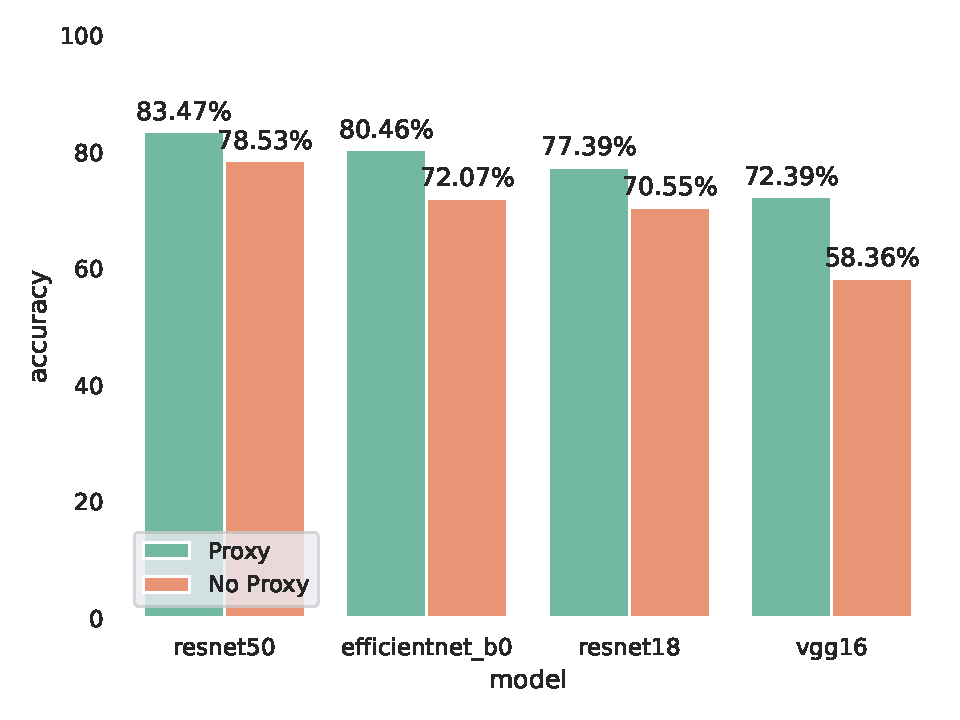
\includegraphics[width=\linewidth, right]{results/tsing_results.pdf}
        \caption{Tsinghua Dogs Dataset}
    \end{subfigure}
    % \hfill
    \begin{subfigure}[h]{.5\textwidth}
        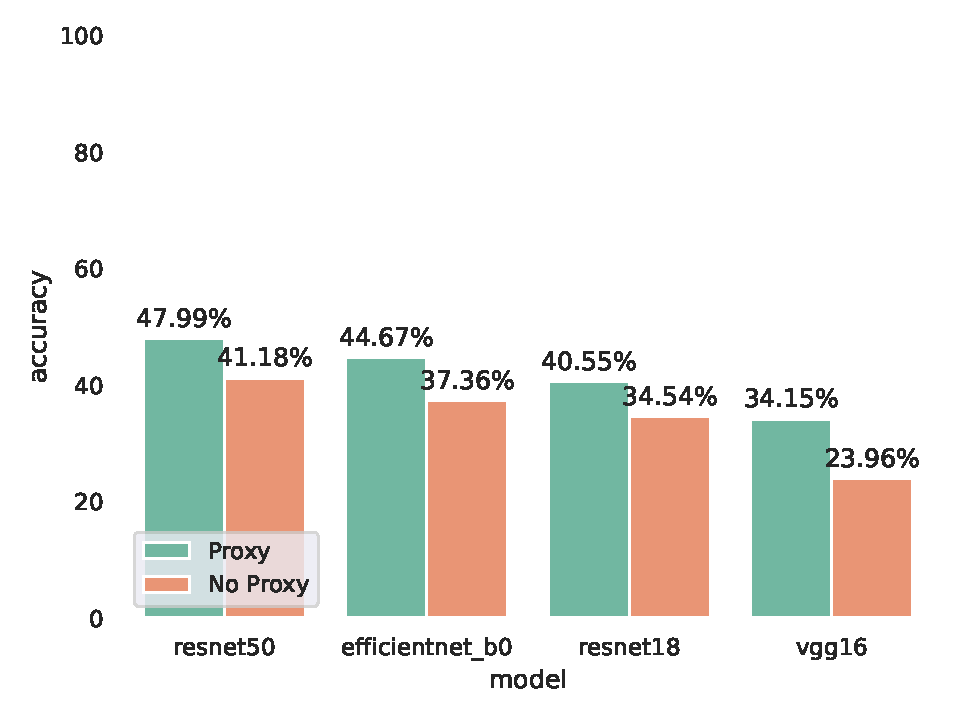
\includegraphics[width=\linewidth, left]{results/places256_results.pdf}
        \caption{Places256 Dataset}
    \end{subfigure}
    \caption{Comparing Accuracies of Models trained with and without Proxy Attention on the Tsinghua Dogs and Places256 datasets}
    \label{fig:tsing_places256_results}
\end{figure}

\subsection{Stanford Dogs and CIFAR100 Results}
This section shows the accuracies per model for the Stanford Dogs \cite{khoslaNovelDatasetFineGrained} and CIFAR100 \cite{krizhevskyLearningMultipleLayers} datasets. The results are shown in Figure \ref{fig:dogs_cifar100_results}.

Like the previous subsection, we can see that the models trained with Proxy Attention outperform the models trained without Proxy Attention. The VGG16 model here was replaced with a vision transformer model for diversity in the results. 

We see that the vision transformer model performs the worst on both datasets while ResNet50 performs the best. This is not to say that vision transformers are bad, but rather that in the same amount of training time, the vision transformer model was not able to learn as much as the other models. 
While the vision transformer initially performed badly, using Proxy Attention was able to improve its performance to be comparable to the performance of the other networks. This goes to show that Proxy Attention can also be used on vision transformer models to improve their performance.
\begin{figure}[!htb]
    % \centering
    \begin{subfigure}[h]{.5\textwidth}
        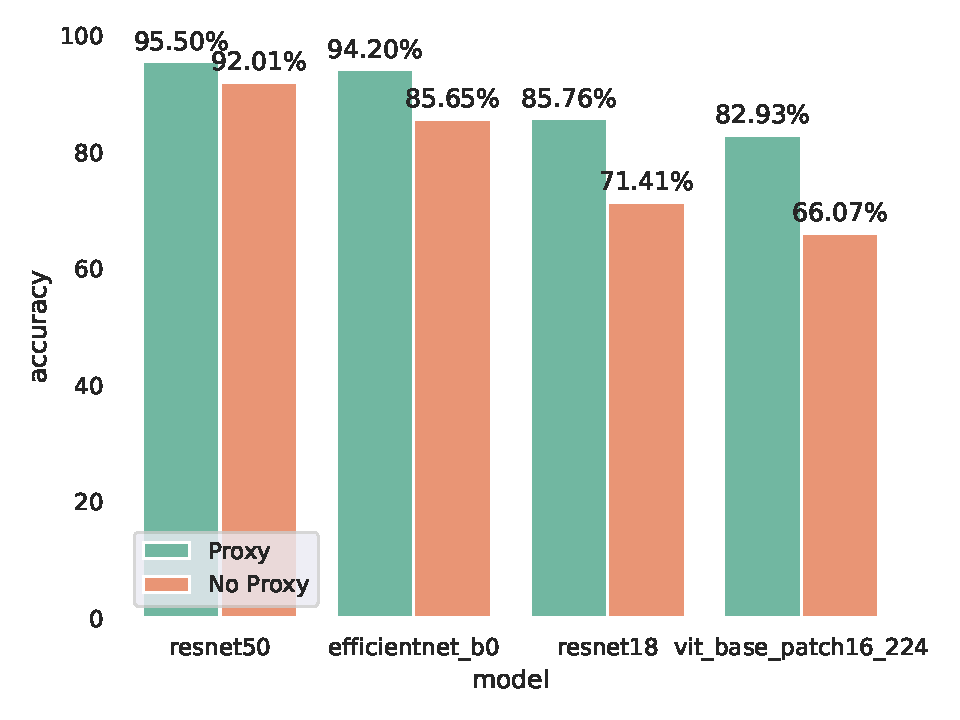
\includegraphics[width=\linewidth, right]{results/dogs_results.pdf}
        \caption{Stanford Dogs Dataset}
    \end{subfigure}
    % \hfill
    \begin{subfigure}[h]{.5\textwidth}
        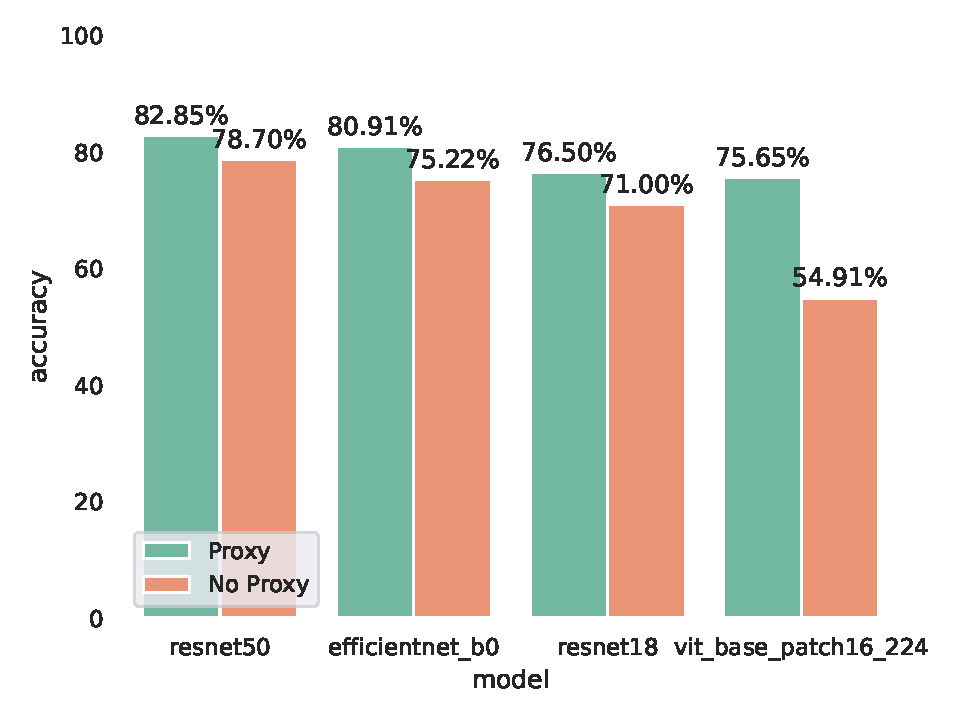
\includegraphics[width=\linewidth, left]{results/cifar100_results.pdf}
        \caption{CIFAR100 Dataset}
    \end{subfigure}
    \caption{Comparing Accuracies of models trained with and without Proxy Attention on the Stanford Dogs and CIFAR100 datasets}
    \label{fig:dogs_cifar100_results}
\end{figure}

\subsection{Caltech101 and ASL Results}
This section shows the accuracies per model for the Caltech101 \cite{liCaltech101} and \href{https://www.kaggle.com/datasets/grassknoted/asl-alphabet}{ASL} datasets. The results are shown in Figure \ref{fig:caltech101_asl_results}.

As before, we can see that the models trained with Proxy Attention outperform those trained without Proxy Attention but the difference is not as large as the previous datasets. This could be because the Caltech101 and ASL datasets are much easier to learn than the previous datasets and thus the original models were already at a high accuracy. That being said, there was still a small improvement in accuracy for the models trained with Proxy Attention. In the odd case of the ASL dataset, the ResNet18 model trained with Proxy Attention performed worse than the model trained without Proxy Attention. Maybe this is because the ASL dataset was the easiest dataset to learn of the ones used in this thesis and thus using Proxy Attention was not necessary and hurt the performance of the model slightly.

\begin{figure}[!htb]
    % \centering
    \begin{subfigure}[h]{.5\textwidth}
        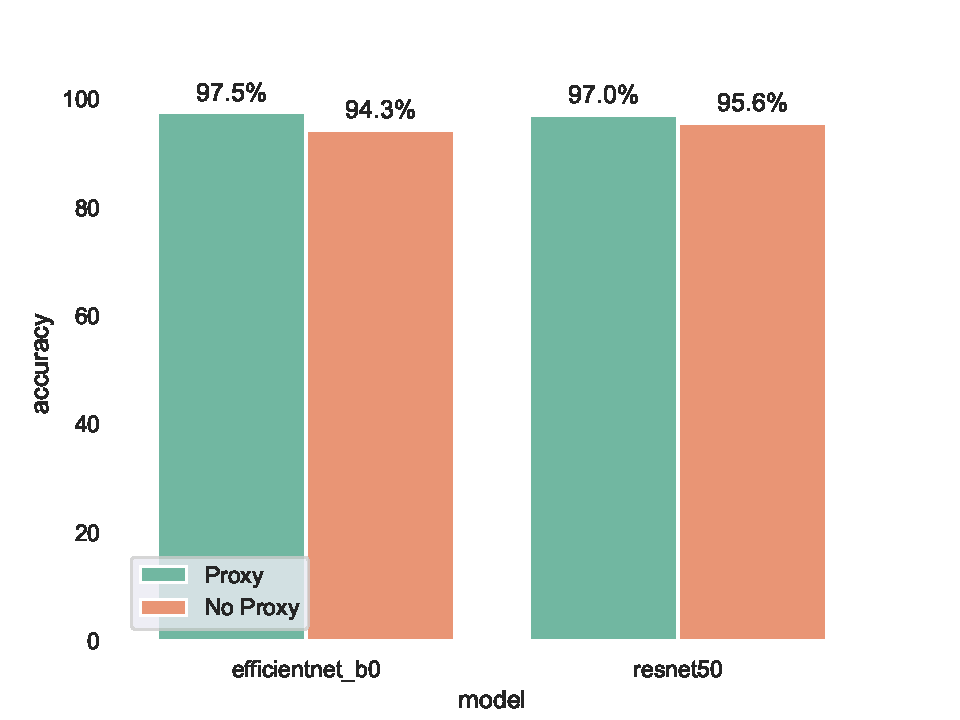
\includegraphics[width=\linewidth, right]{results/caltech101_results.pdf}
        \caption{Caltech101 Dataset}
    \end{subfigure}
    % \hfill
    \begin{subfigure}[h]{.5\textwidth}
        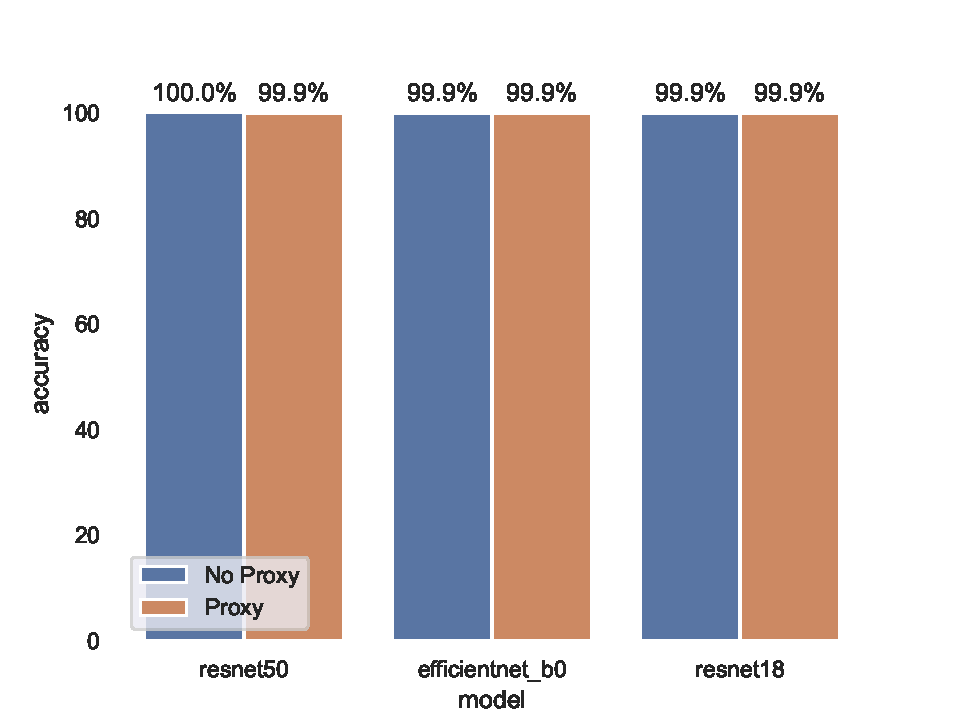
\includegraphics[width=\linewidth, left]{results/asl_results.pdf}
        \caption{Asl Dataset}
    \end{subfigure}
    \caption{Comparing Accuracies of models trained with and without Proxy Attention on the Caltech101 and Asl datasets}
    \label{fig:caltech101_asl_results}
\end{figure}

\subsection{Plant Disease Results}
This section shows the accuracies per model for the \href{https://www.kaggle.com/datasets/rajibdpi/plant-disease-dataset}{Plant Disease} dataset. The results are shown in Figure \ref{fig:plantdisease_results}. 

The plant disease dataset is also of a similar difficulty to the Caltech101 and ASL datasets and thus the models trained with Proxy Attention did not perform much better than the models trained without Proxy Attention. Although in most cases there was some improvement after using Proxy Attention, the ResNet50 model seemed to do better in the case where Proxy Attention was not used. 
\begin{figure}[!htb]
    \centering
    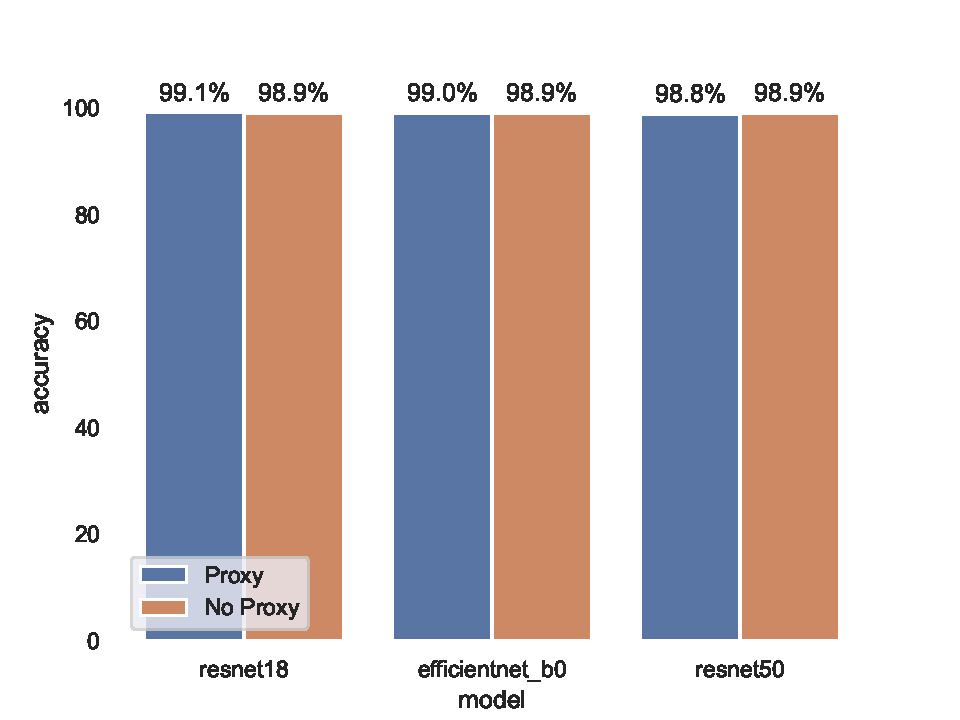
\includegraphics[width=.6\linewidth]{results/plantdisease_results.pdf}
    \caption{Comparing Accuracies of models trained with and without Proxy Attention on the Plant Disease dataset}
    \label{fig:plantdisease_results}
\end{figure}


\subsection{Results Grouped By Schedule}
This section explores the validation accuracy obtained for different step schedules. The results are shown in Figure \ref{fig:schedresnet50_results}. 
There were three types of schedules tested in this thesis: no proxy, proxy applied after half the training steps ([20, 'p',19]), and proxy applied every couple of steps ([5, 'p', 9, 'p',9, 'p',4]). The total number of training steps was 40 for all schedules with every network trained with and without Proxy Attention being given the same parameters. 

We can see that the models trained with Proxy Attention outperform the models trained without Proxy Attention for all three schedules. The schedule that performed the best was the schedule that applied Proxy Attention every couple of steps. This could be because the model was able to learn more from the Proxy Attention module when it was applied more often. While applying the proxy step in the middle of training was also able to improve the performance of the model, it can be seen that applying the proxy step multiple times was able to improve the performance even more.
\begin{figure}[!htb]
    \centering
    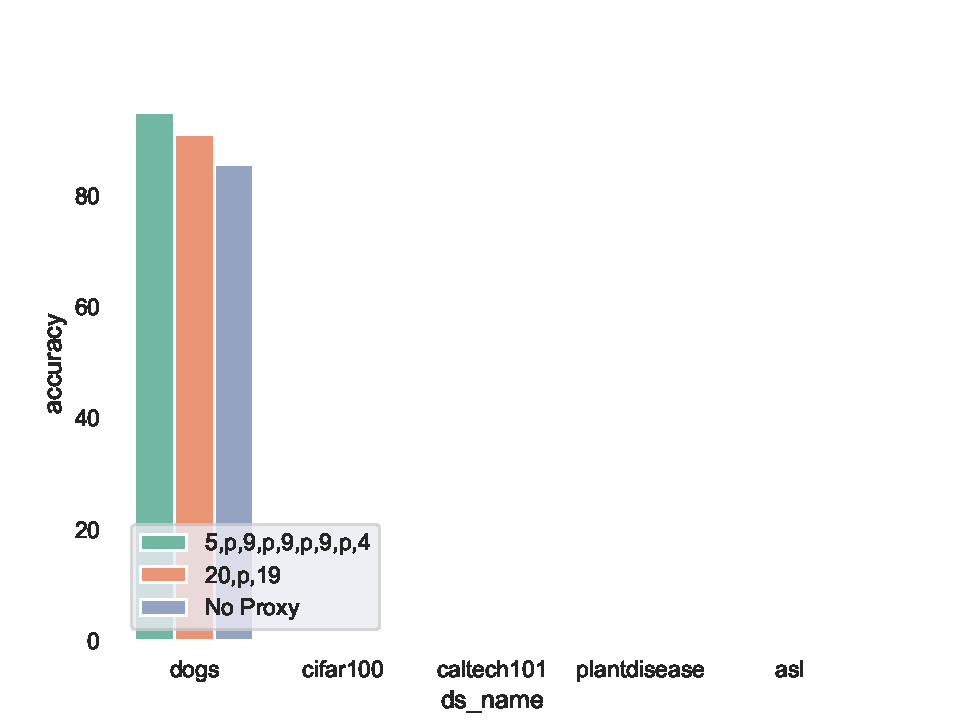
\includegraphics[width=.6\textwidth]{results/schedule_resnet50.pdf}
    \caption{Comparing Accuracies of models trained with and without Proxy Attention on the ResNet50 \cite{heDeepResidualLearning2016} architecture for different step schedules}.
    \label{fig:schedresnet50_results}
\end{figure}

\subsection{Results Grouped By Proxy Threshold}
This section explores the validation accuracy obtained for different Proxy thresholds. The results are shown in Figure \ref{fig:proxy_threshold}. 
The comparison was done for two different datasets: the Stanford Dogs dataset \cite{khoslaNovelDatasetFineGrained} and the Tsinghua Dogs dataset \cite{zouNewDatasetDog2020}. While the Stanford Dogs dataset is a relatively easy dataset to learn, the Tsinghua Dogs dataset is a much harder dataset to learn and thus these two datasets were chosen to see how the Proxy Threshold affects the performance of the model for datasets of different complexities. Since the comparison is done for the Proxy Threshold, different models were chosen to identify the best value across different architectures and datasets. Thus for these two figures, only comparing the value of the Proxy Threshold is important and not the actual accuracy of the model.

The results are not conclusive for this comparison and it can be said that the Proxy Threshold remains a hyperparameter that needs to be tuned for each dataset.
For the EfficientNetB0 \cite{tanEfficientnetRethinkingModel2019} trained with Proxy Attention on the Stanford Dogs dataset\cite{khoslaNovelDatasetFineGrained}, the best Proxy Threshold was 0.8, while the others had a similar performance. For the Resnet18 \cite{heDeepResidualLearning2016} trained with Proxy Attention on the Tsinghua Dogs Dataset \cite{zouNewDatasetDog2020}, the best Proxy Threshold was 0.1 and 0.85, while the others had a similar performance.
In this case, choosing a value of 0.85 for the Proxy Threshold would be a good starting point, and further tuning could be done to improve the performance of the model if needed.

\begin{figure}[!htb]
    \begin{subfigure}[h]{.5\textwidth}
        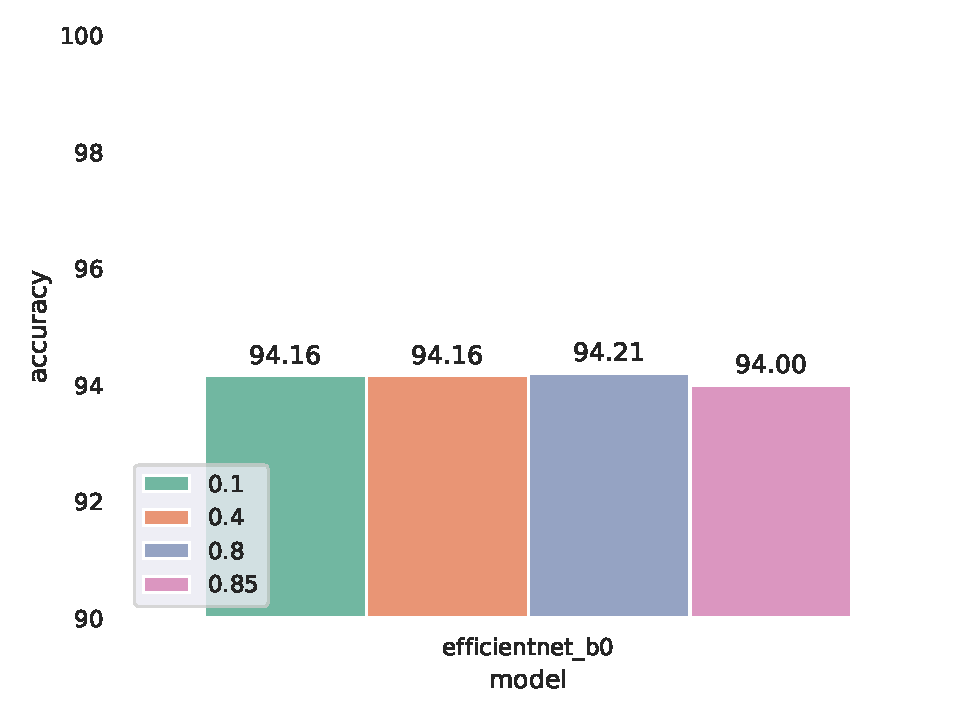
\includegraphics[width=\linewidth, right]{results/proxy_threshold_results.pdf}
        \caption{EfficientNetB0 \cite{tanEfficientnetRethinkingModel2019} trained with Proxy Attention on the Stanford Dogs dataset\cite{khoslaNovelDatasetFineGrained}}
    \end{subfigure}
    % \hfill
    \begin{subfigure}[h]{.5\textwidth}
        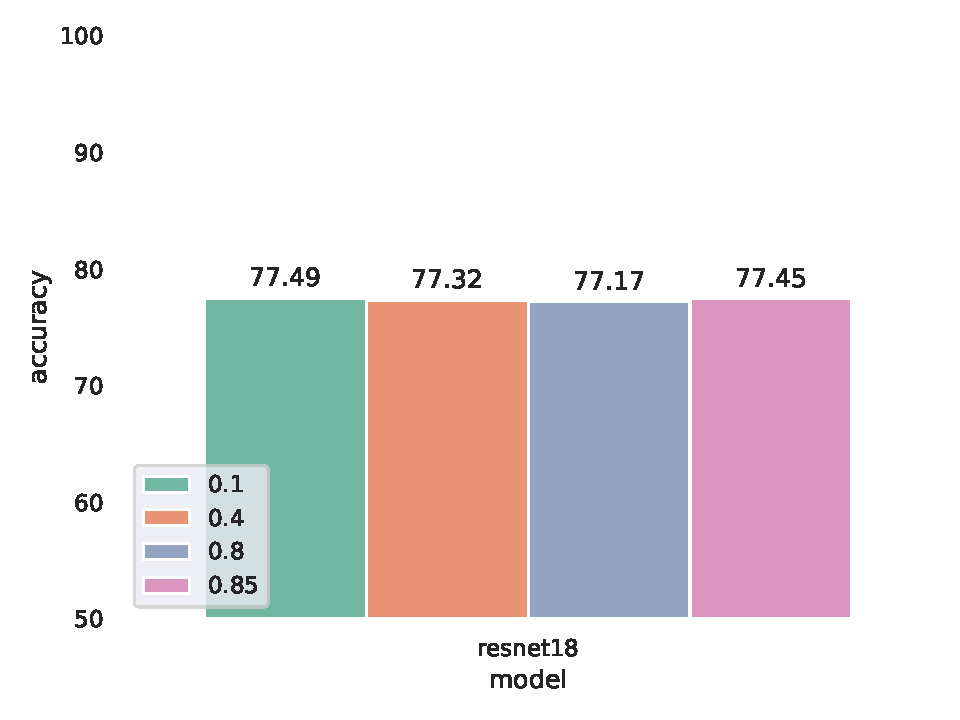
\includegraphics[width=\linewidth, left]{results/proxy_threshold_results_tsing.pdf}
        \caption{Resnet18 \cite{heDeepResidualLearning2016} trained with Proxy Attention on the Tsinghua Dogs Dataset \cite{zouNewDatasetDog2020}}
    \end{subfigure}
    
    \caption{Comparing Accuracies of models trained with Proxy Attention for Different Proxy Thresholds}
    \label{fig:proxy_threshold}
\end{figure}

\subsection{Results Grouped By Proxy Image Weight}
This section explores the validation accuracy obtained for different Proxy image weights. The results are shown in Figure \ref{fig:proxy_weight}. 
The comparison was done for two different datasets: the Stanford Dogs dataset \cite{khoslaNovelDatasetFineGrained} and the Tsinghua Dogs dataset \cite{zouNewDatasetDog2020}. While the Stanford Dogs dataset is a relatively easy dataset to learn, the Tsinghua Dogs dataset is a much harder dataset to learn and thus these two datasets were chosen to see how the Proxy Image Weight affects the performance of the model for datasets of different complexities. Since the comparison is done for the Proxy Image Weight, different models were chosen to identify the best value across different architectures and datasets. Thus for these two figures, only comparing the value of the Proxy Image Weight is important and not the actual accuracy of the model.

For the EfficientNetB0 \cite{tanEfficientnetRethinkingModel2019} trained with Proxy Attention on the Stanford Dogs dataset\cite{khoslaNovelDatasetFineGrained}, the best Proxy Image Weight was 0.1, while the others had a similar performance except for a weight of 0.2 which performed the worst. For the Resnet18 \cite{heDeepResidualLearning2016} trained with Proxy Attention on the Tsinghua Dogs Dataset \cite{zouNewDatasetDog2020}, the best Proxy Image Weight were 0.4 and 0.8, while the others had a similar performance.
While the results are not fully conclusive, using a Proxy Image Weight of 0.1 or 0.4 seems to be a good choice. Further, tuning is always recommended if required.

\begin{figure}[!htb]
    \begin{subfigure}[h]{.5\textwidth}
        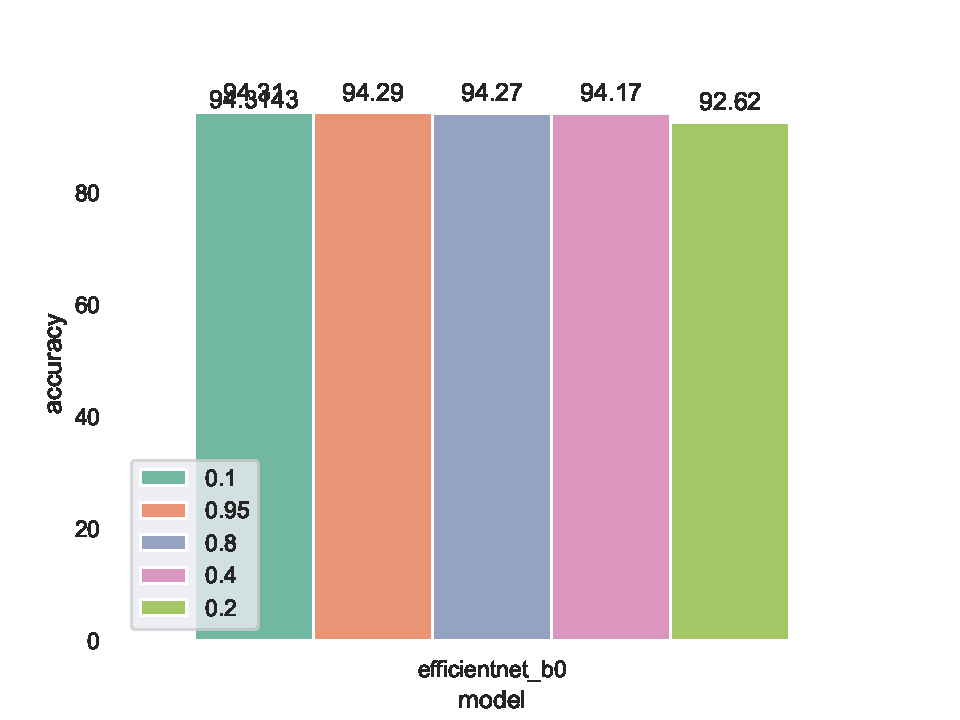
\includegraphics[width=\linewidth, right]{results/proxy_weight_results.pdf}
        \caption{EfficientNetB0 \cite{tanEfficientnetRethinkingModel2019} trained with Proxy Attention on the Stanford Dogs dataset\cite{khoslaNovelDatasetFineGrained}}
    \end{subfigure}
    % \hfill
    \begin{subfigure}[h]{.5\textwidth}
        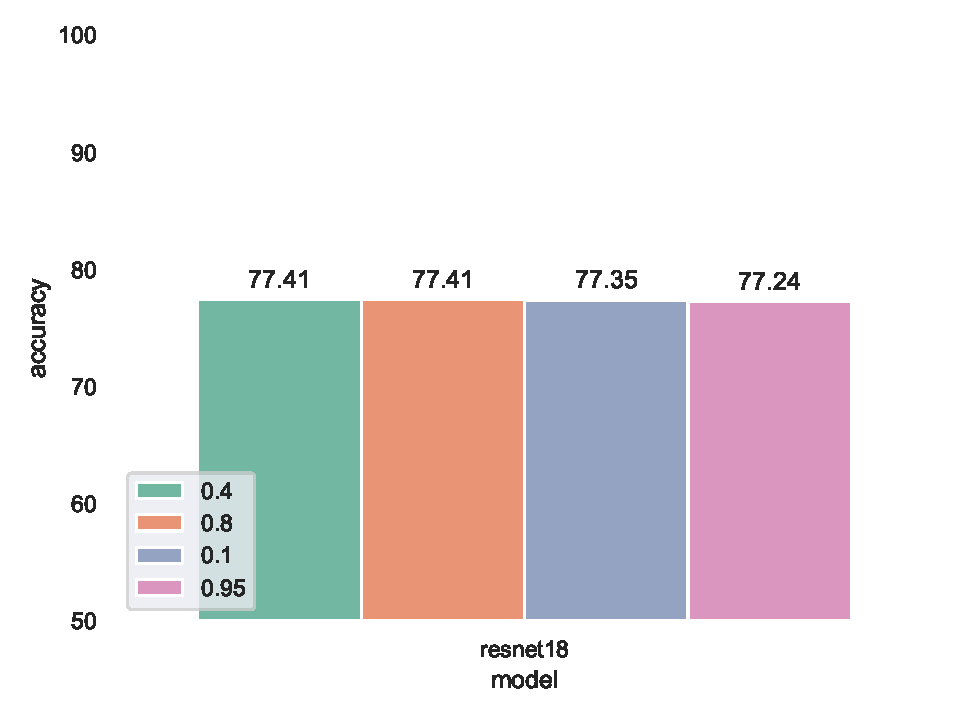
\includegraphics[width=\linewidth, left]{results/proxy_weight_results_tsing.pdf}
        \caption{Resnet18 \cite{heDeepResidualLearning2016} trained with Proxy Attention on the Tsinghua Dogs Dataset \cite{zouNewDatasetDog2020}}
    \end{subfigure}
    
    \caption{Comparing Accuracies of models trained with Proxy Attention for Different Proxy Image Weights}
    \label{fig:proxy_weight}
\end{figure}

\subsection{Results Grouped By Proxy Image Subset}
This section explores the validation accuracy obtained for different Proxy image subsets. The results are shown in Figure \ref{fig:proxy_subset}.
The comparison was done for two different datasets: the Stanford Dogs dataset \cite{khoslaNovelDatasetFineGrained} and the Tsinghua Dogs dataset \cite{zouNewDatasetDog2020}. While the Stanford Dogs dataset is a relatively easy dataset to learn, the Tsinghua Dogs dataset is a much harder dataset to learn and thus these two datasets were chosen to see how the Proxy Image Subset affects the performance of the model for datasets of different complexities. Since the comparison is done for the Proxy Image Subset, different models were chosen to identify the best value across different architectures and datasets. Thus for these two figures, only comparing the value of the Proxy Image Subset is important and not the actual accuracy of the model.

For the EfficientNetB0 \cite{tanEfficientnetRethinkingModel2019} trained with Proxy Attention on the Stanford Dogs dataset\cite{khoslaNovelDatasetFineGrained}, the best Proxy Image Subset was 0.2 and 0.95, while the others had a similar performance except for a subset of 0.8 which performed the worst. For the Resnet18 \cite{heDeepResidualLearning2016} trained with Proxy Attention on the Tsinghua Dogs Dataset \cite{zouNewDatasetDog2020}, the best Proxy Image Subset were 0.2 and 0.95, while 0.8 performed the worst.

Tuning the Proxy Image Subset seems to give significant improvements as compared to tuning the others, thus it is recommended to tune the Proxy Image Subset first before tuning the others. A good starting point would be to use a Proxy Image Subset of 0.2. Further, tuning is always recommended if required.
It is also interesting to note that in the case of the EfficientNetB0 \cite{tanEfficientnetRethinkingModel2019} trained with Proxy Attention on the Stanford Dogs dataset\cite{khoslaNovelDatasetFineGrained}, the model already performed quite well, and thus adding more Proxy Images did more harm than good. While in the case of the Resnet18 \cite{heDeepResidualLearning2016} trained with Proxy Attention on the Tsinghua Dogs Dataset \cite{zouNewDatasetDog2020}, the model did not perform as well, and thus adding more Proxy Images did not degrade the performance but rather improved it.

\begin{figure}[!htb]
    \begin{subfigure}[h]{.5\textwidth}
        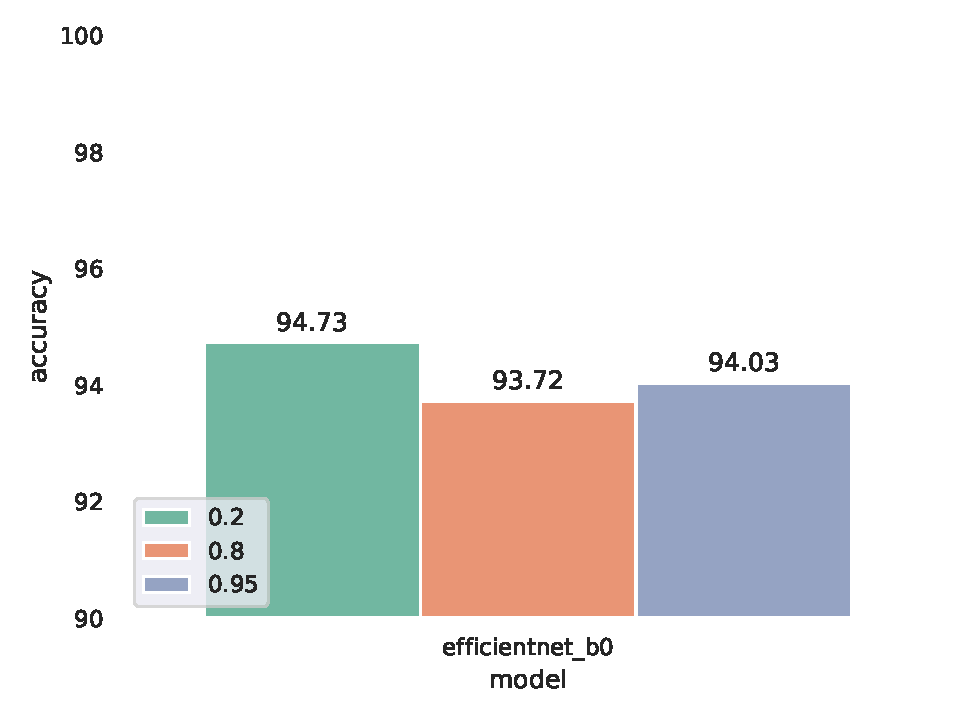
\includegraphics[width=\linewidth, right]{results/proxy_subset_attention_results.pdf}
        \caption{EfficientNetB0 \cite{tanEfficientnetRethinkingModel2019} trained with Proxy Attention on the Stanford Dogs dataset\cite{khoslaNovelDatasetFineGrained}}
    \end{subfigure}
    % \hfill
    \begin{subfigure}[h]{.5\textwidth}
        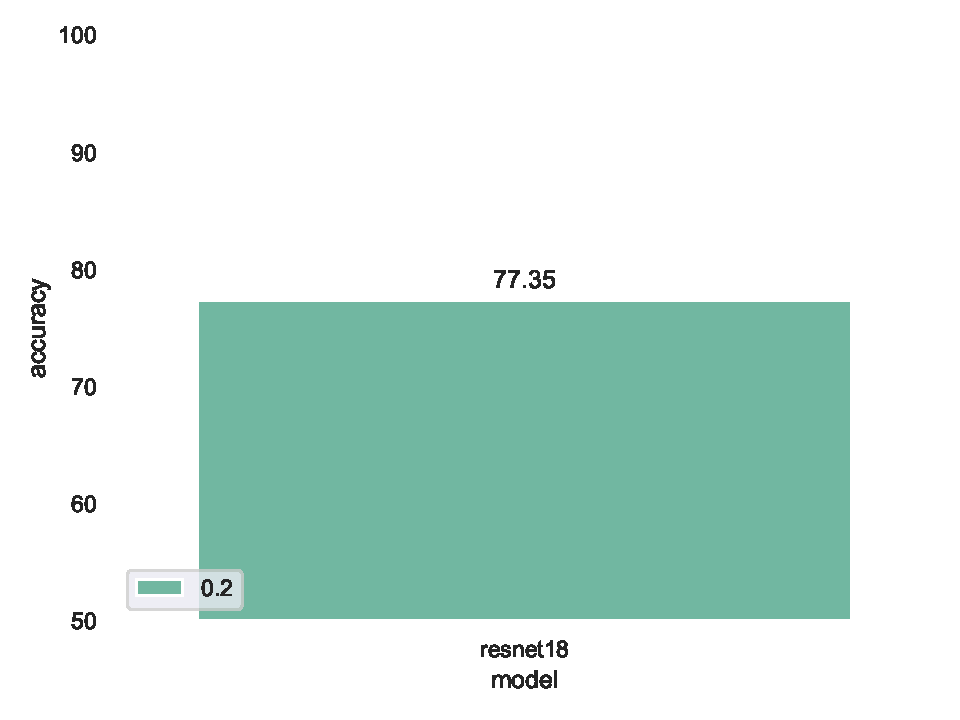
\includegraphics[width=\linewidth, left]{results/proxy_subset_results_tsing.pdf}
        \caption{Resnet18 \cite{heDeepResidualLearning2016} trained with Proxy Attention on the Tsinghua Dogs Dataset \cite{zouNewDatasetDog2020}}
    \end{subfigure}
    
    \caption{Comparing Accuracies of models trained with Proxy Attention for different Proxy Image Subsets}
    \label{fig:proxy_subset}
\end{figure}

\section{Explanability}
This section explores the explainability of the models for different hyperparameters and datasets by using a trained model to generate attention maps for a given input image. The attention maps are compared between the same network (with the same hyperparameters) trained with and without Proxy Attention. For explanations of the results demonstrated in the section, please refer to the discussion section ~\ref{ch:discussion}.

\subsection{CIFAR 100, ResNet18, EigenGradCAM}
This section explores the explainability of the Resnet18 \cite{heDeepResidualLearning2016} trained with and without Proxy Attention on the cifar100 dataset \cite{krizhevskyLearningMultipleLayers}. The results are shown in Figure \ref{fig:resnet18_cifar100}. The attention maps were generated using EigenGradCAM \cite{banymuhammadEigenCAMVisualExplanations2021}.

Here we can see that, for most of the images, there is no difference between the predictions of the proxy attention method and the original prediction. For some of the images, such as the cockroach and the snake, the original prediction was correct, but the prediction after applying the proxy method turned out to be wrong. This does show that using proxy attention does not negatively affect the attention of the model in most cases but occasionally it does. 

\begin{figure}[!htb]
    \begin{subfigure}[b]{1\textwidth}
        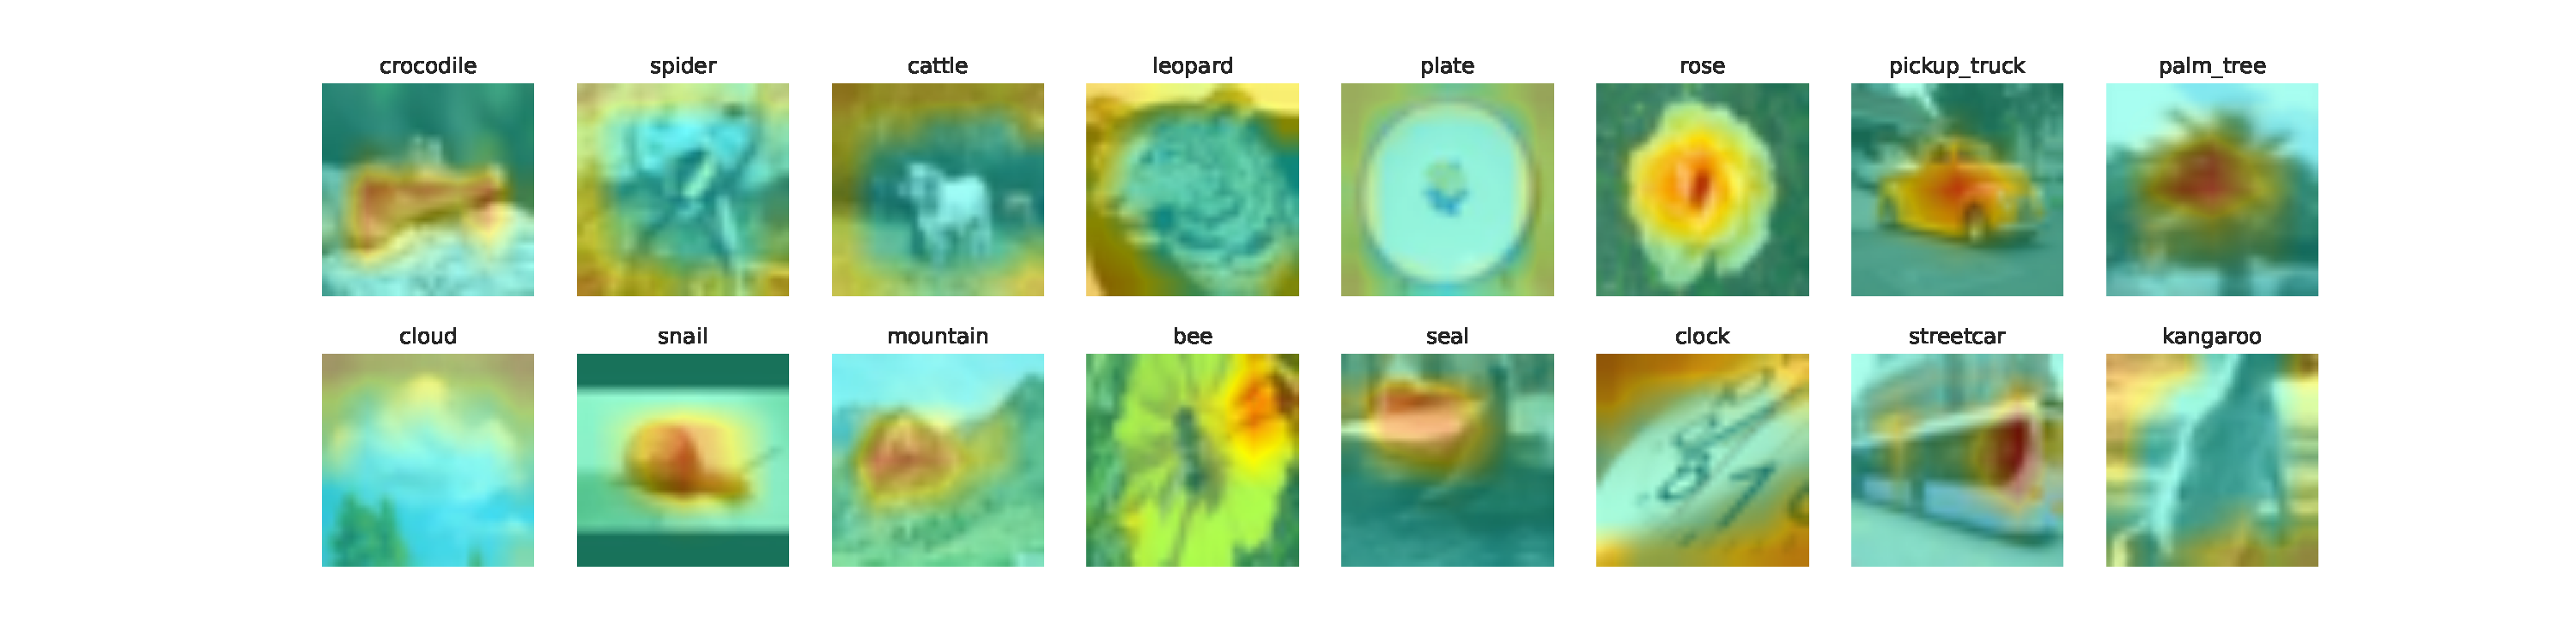
\includegraphics[width=\linewidth]{images/cifar100_resnet18_noproxy_0.pdf}
        \caption{Without Proxy Attention}
    \end{subfigure}
    \begin{subfigure}[b]{1\textwidth}
        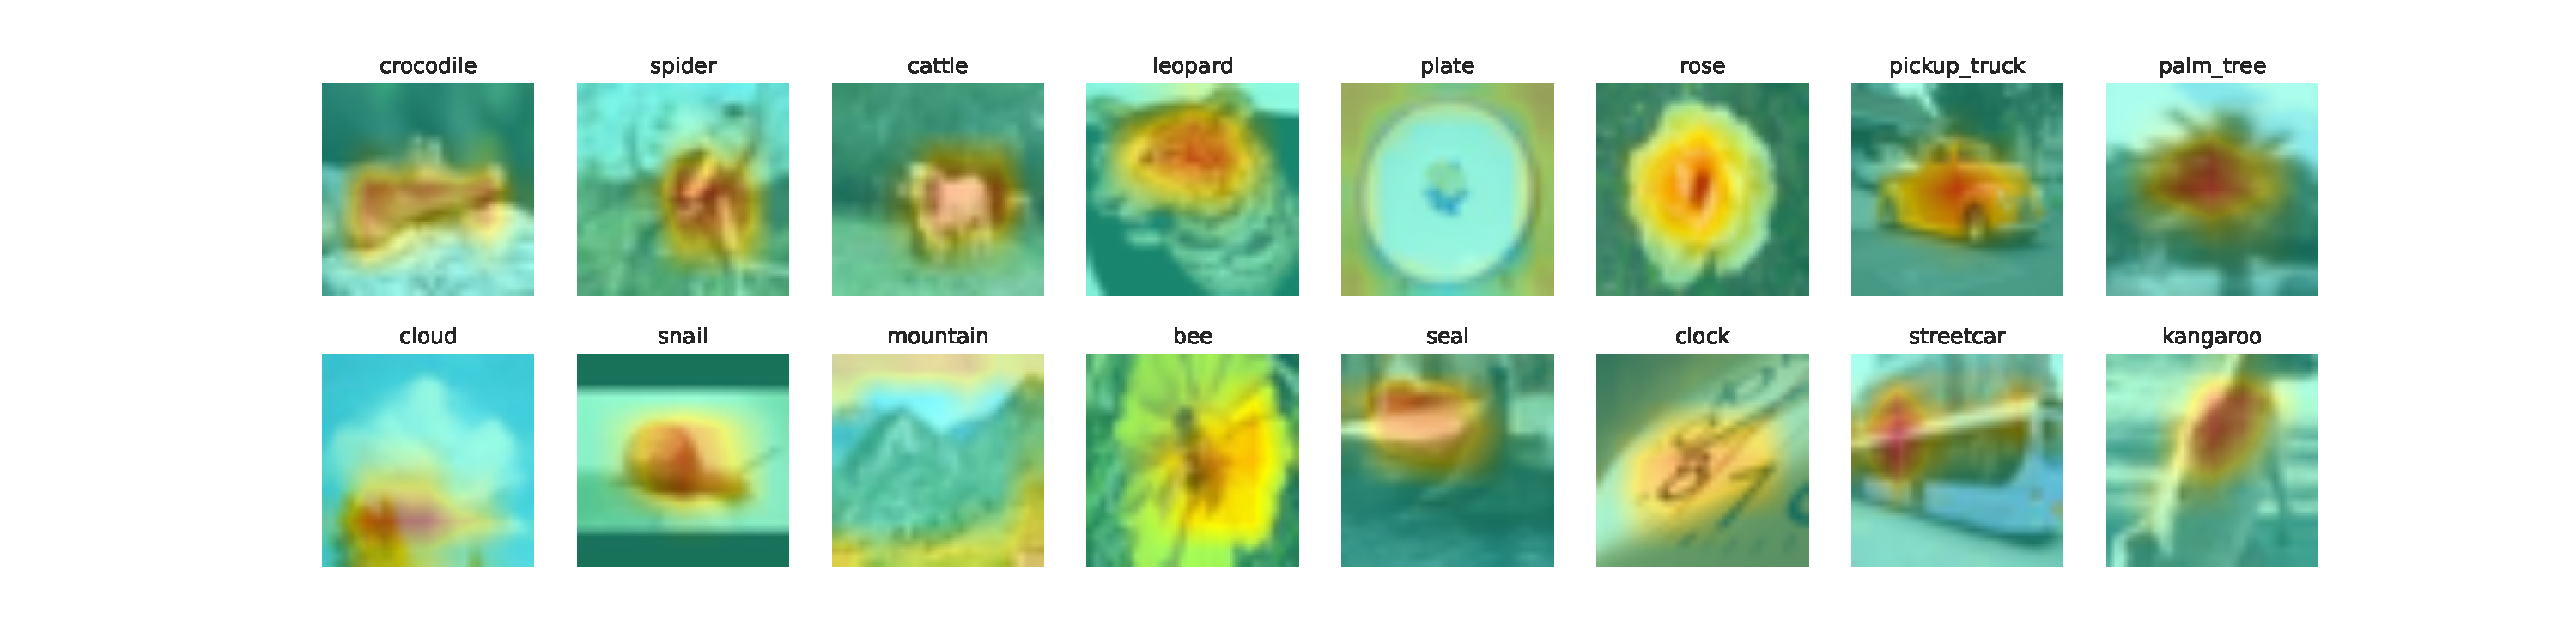
\includegraphics[width=\linewidth]{images/cifar100_resnet18_proxy_0.pdf}
        \caption{With Proxy Attention}
    \end{subfigure}
    
    \caption{Comparison of attention maps generated by resnet18 trained with and without Proxy Attention on the cifar100 dataset}
    \label{fig:resnet18_cifar100}
\end{figure}


\subsection{CIFAR 100, EfficientNetB0, EigenGradCAM}
This section explores the explainability of the EfficientNetB0 \cite{tanEfficientnetRethinkingModel2019} trained with and without Proxy Attention on the cifar100 dataset \cite{krizhevskyLearningMultipleLayers}. The results are shown in Figure \ref{fig:efficientnet_b0_cifar100}. The attention maps were generated using EigenGradCAM \cite{banymuhammadEigenCAMVisualExplanations2021}.

For this comparison, it seems that the networks predicted the results quite accurately. This also shows that using the proxy method did not negatively affect the results. For a single case of the wardrobe, the network that did not use proxy attention seemed to place higher attention on the floor while after using the proxy attention step, the model learned to focus on the wardrobe itself. It is to be noted that in the case of the roads, the model trained with proxy attention seemed to make a mistake.

\begin{figure}[!htb]
    \begin{subfigure}[b]{1\textwidth}
        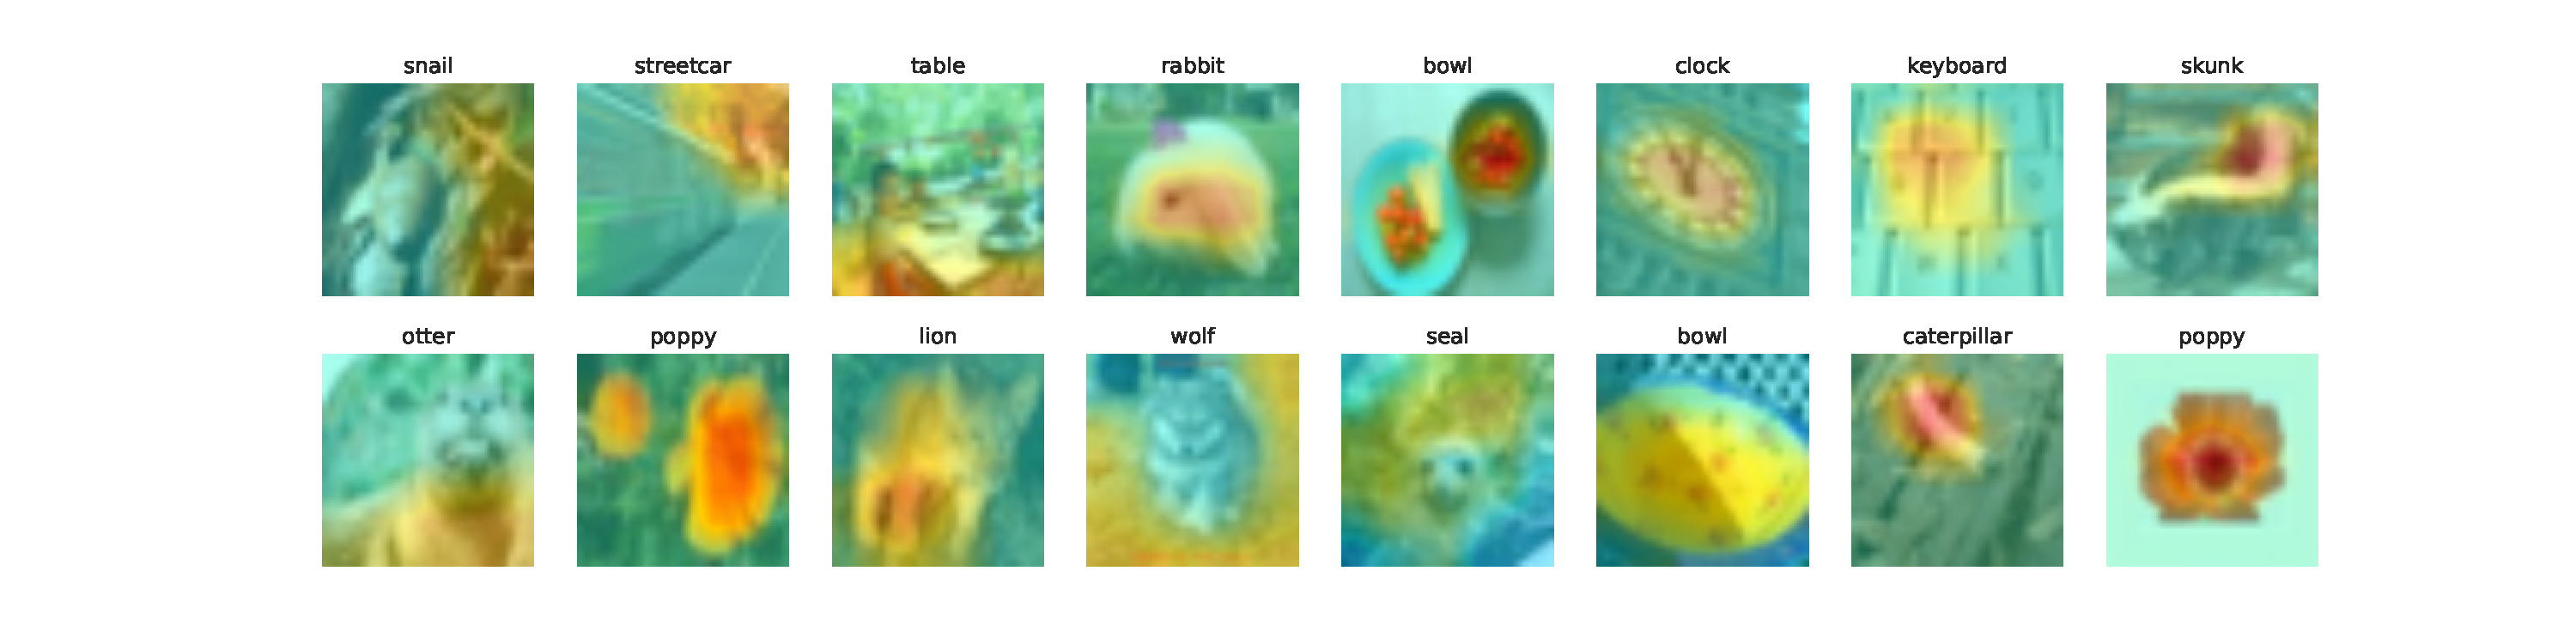
\includegraphics[width=\linewidth]{images/cifar100_efficientnet_b0_noproxy_0.pdf}
        \caption{Without Proxy Attention}
    \end{subfigure}
    \begin{subfigure}[b]{1\textwidth}
        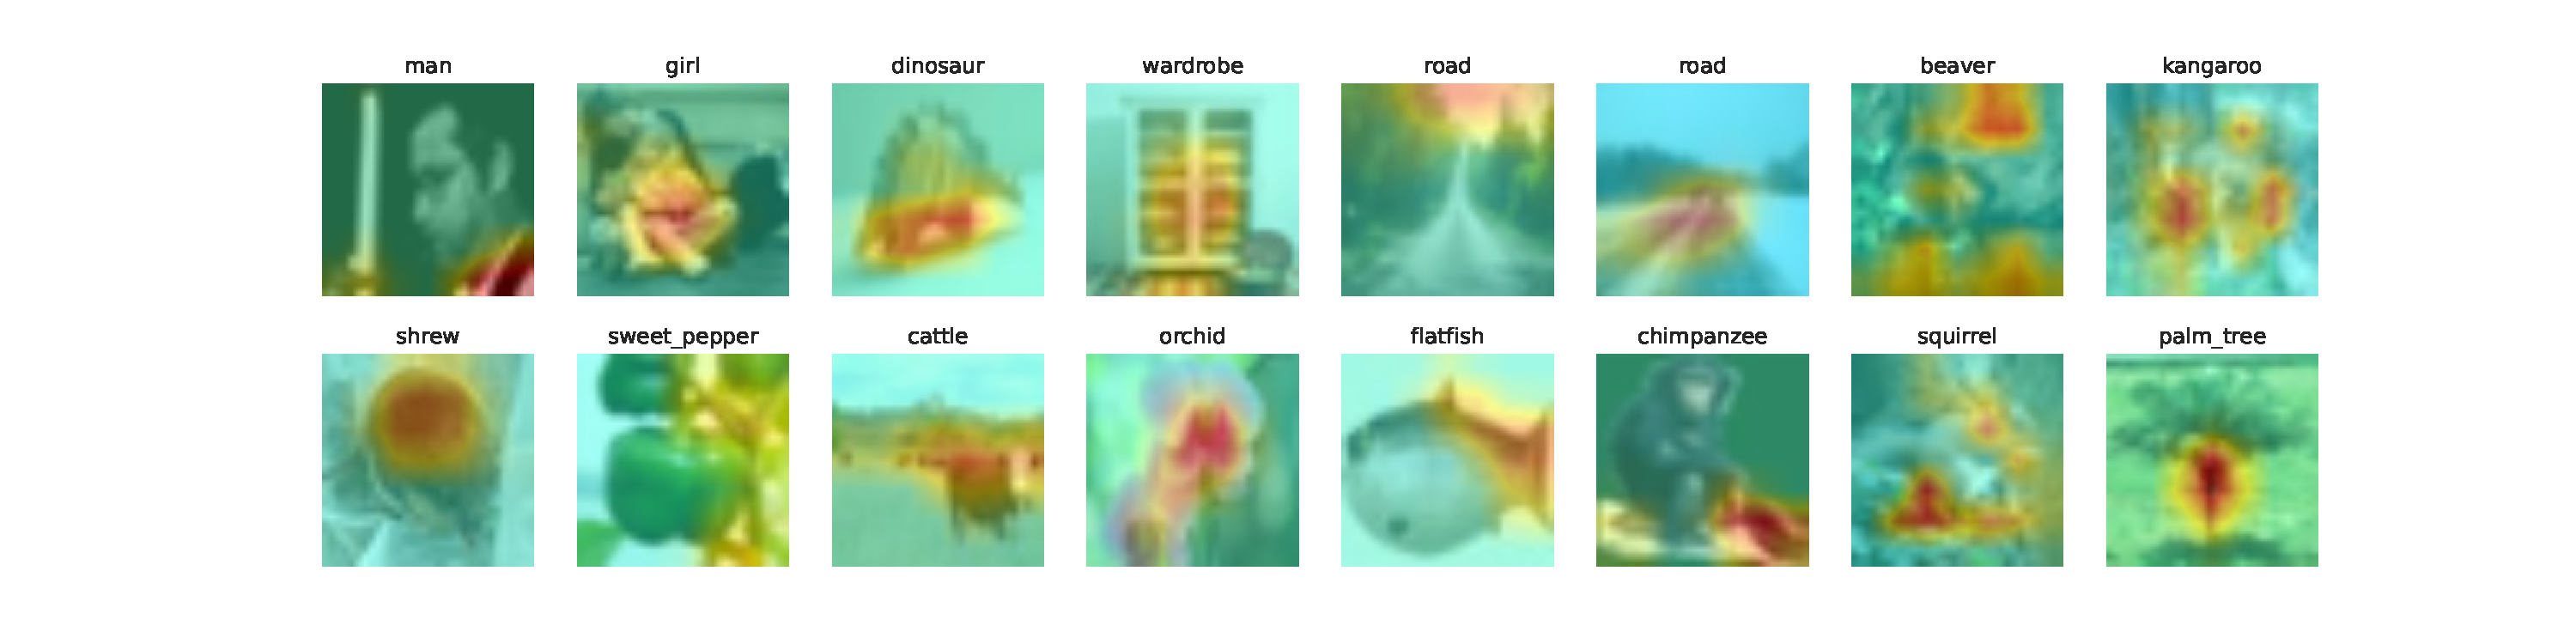
\includegraphics[width=\linewidth]{images/cifar100_efficientnet_b0_proxy_0.pdf}
        \caption{With Proxy Attention}
    \end{subfigure}

    \caption{Comparison of attention maps generated by efficientnet\_b0 trained with and without Proxy Attention on the cifar100 dataset}
    \label{fig:efficientnet_b0_cifar100}
\end{figure}
    


\subsection{CIFAR 100, ViT , EigenGradCAM}
This section explores the explainability of the ViT \cite{dosovitskiyImageWorth16x162021} trained with and without Proxy Attention on the cifar100 dataset \cite{krizhevskyLearningMultipleLayers}. The results are shown in Figure \ref{fig:vit_cifar100}. The attention maps were generated using EigenGradCAM \cite{banymuhammadEigenCAMVisualExplanations2021}.

This comparison is for the vision transformer. Since the transformer network learns the images in patches, and no other preprocessing step was applied, the attention map is denoted as localized points across the image and not complete attention like the CNNs before. In this case, it did seem that using proxy attention, helped the network focus quite a bit on the correct regions of the image. For example, in the lion, man, couch, beaver, et cetera. The model had initially learned the wrong part of the image, but in the case of the proxy intention model, the correct part of the image was learned. Only in the case of the cloud, does it seem that the model trained with proxy attention learned the wrong part of the image.

    \begin{figure}[!htb]
        \begin{subfigure}[b]{1\textwidth}
            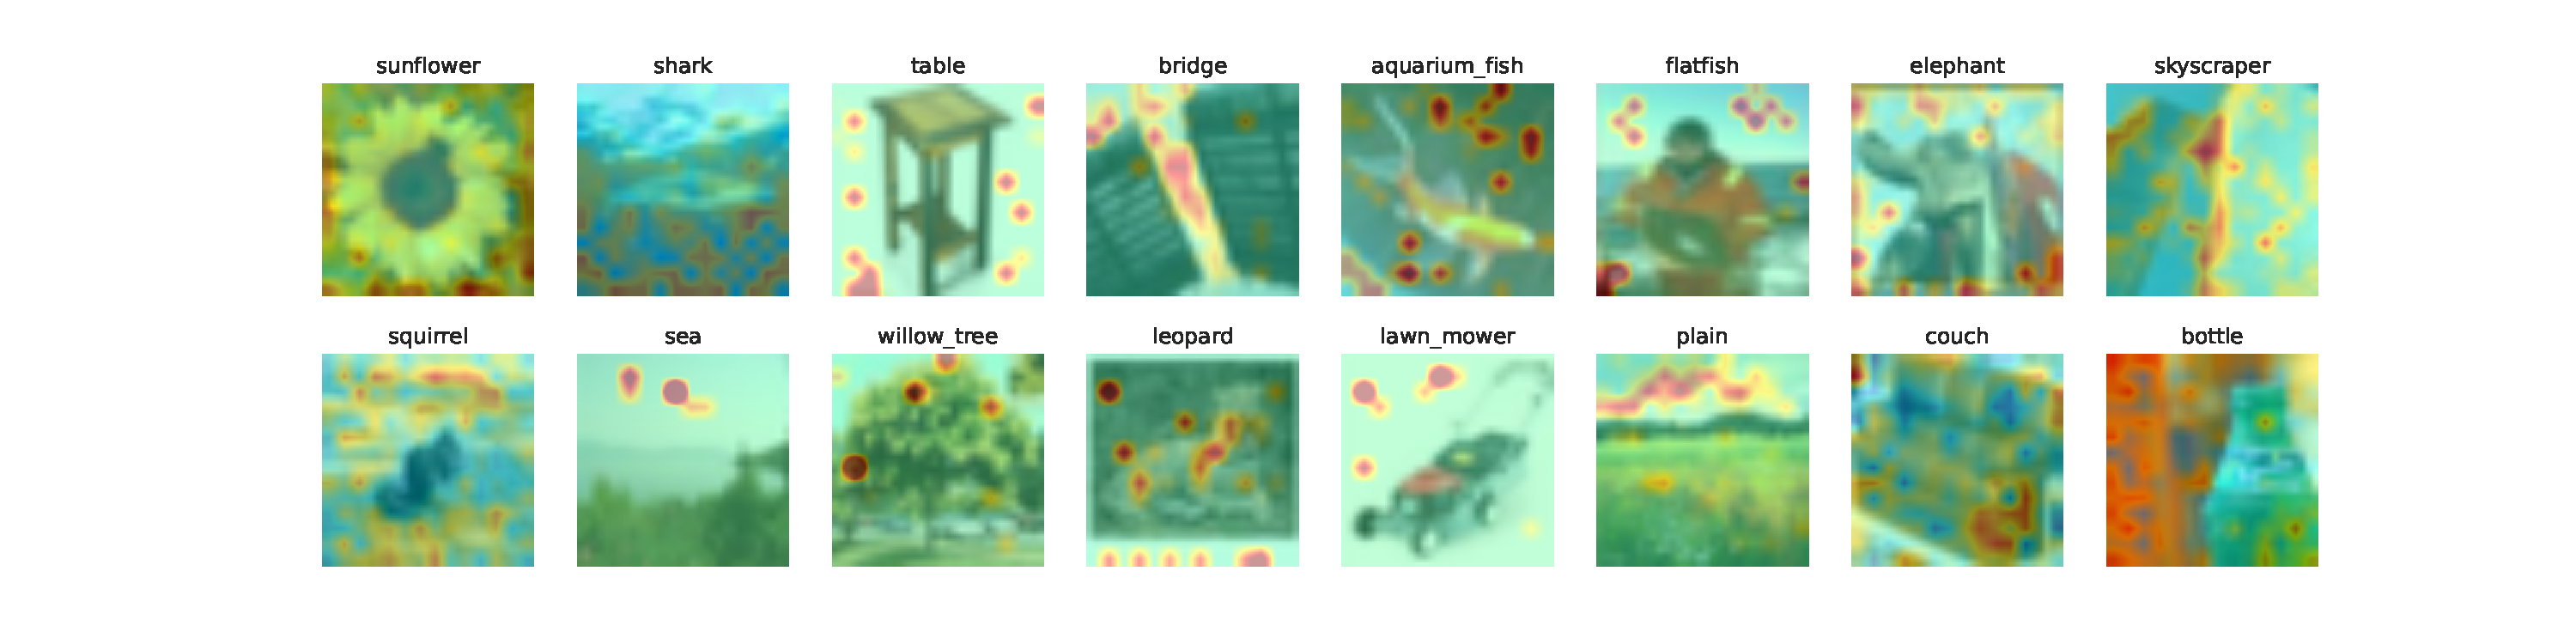
\includegraphics[width=\linewidth]{images/gpp_cifar100_vit_base_patch16_224_noproxy_0.pdf}
            \caption{Without Proxy Attention}
        \end{subfigure}
        \begin{subfigure}[b]{1\textwidth}
            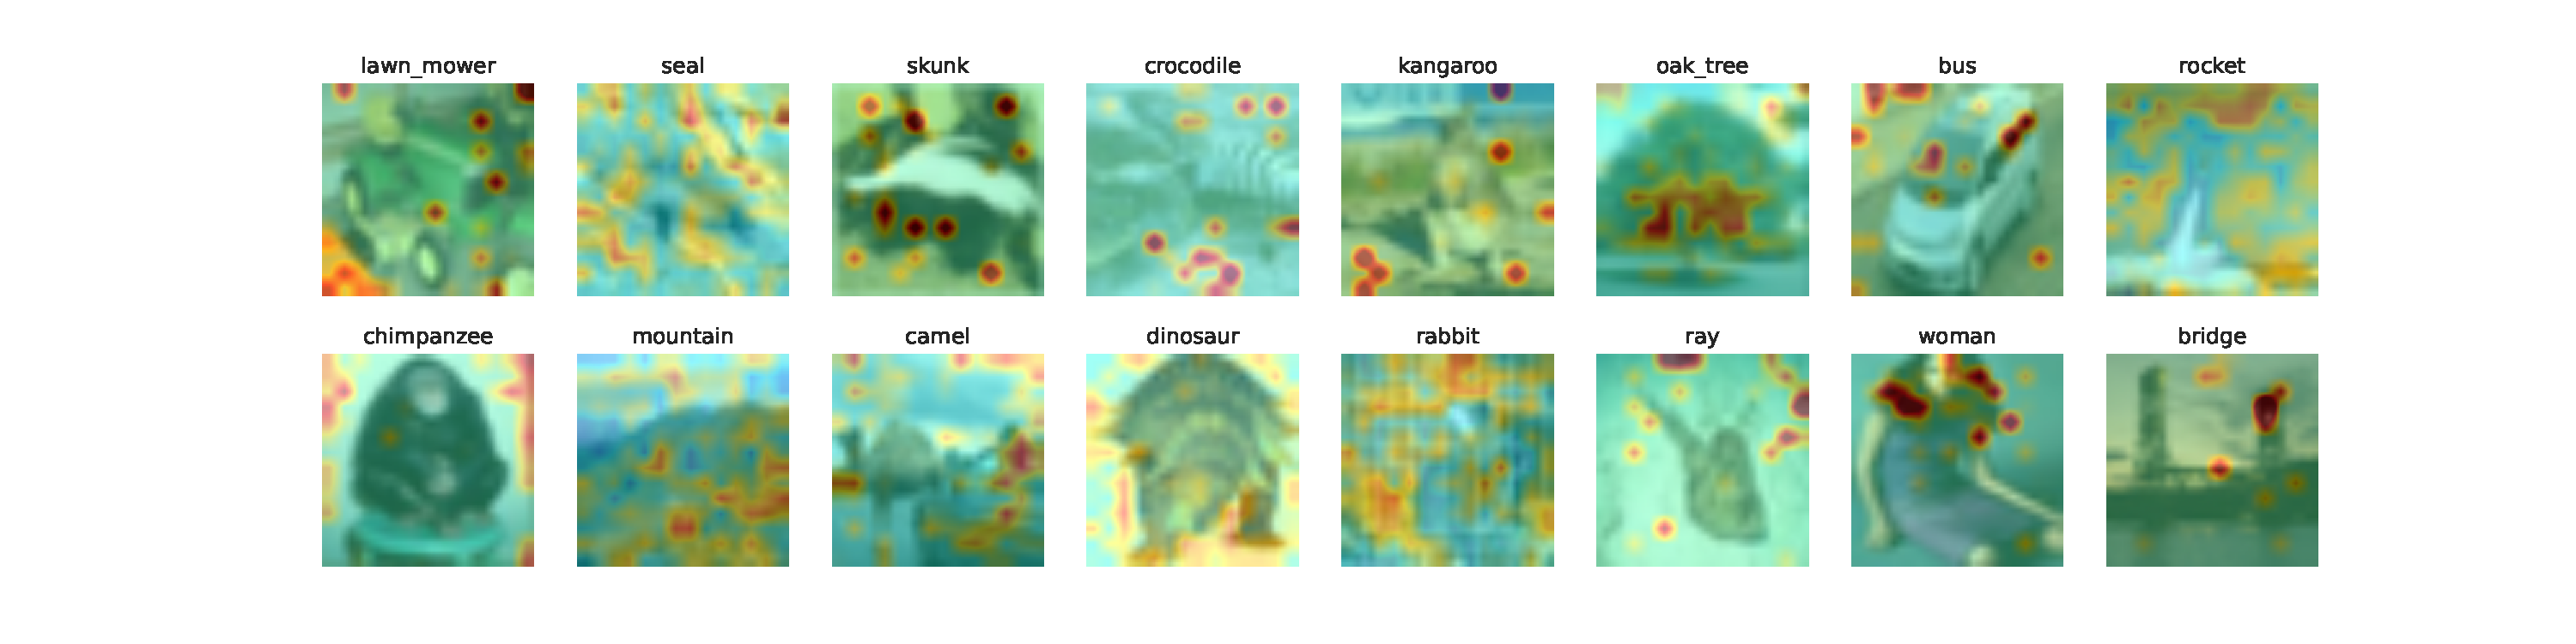
\includegraphics[width=\linewidth]{images/gpp_cifar100_vit_base_patch16_224_proxy_0.pdf}
            \caption{With Proxy Attention}
        \end{subfigure}
        \caption{Comparison of attention maps generated by vit\_base\_patch16\_224 trained with and without Proxy Attention on the cifar100 dataset}
        \label{fig:vit_cifar100}
    \end{figure}
    


\subsection{CIFAR 100, ViT , GradCamPlusPlus}
This section explores the explainability of the ViT \cite{dosovitskiyImageWorth16x162021} trained with and without Proxy Attention on the cifar100 dataset \cite{krizhevskyLearningMultipleLayers}. The results are shown in Figure \ref{fig:vit_cifar100}. The attention maps were generated using GradCamPlusPlus \cite{chattopadhayGradCAMGeneralizedGradientBased2018}.

The results of this comparison are similar to the one above. In the case of the possum, the man had to try the model relearnt the attention map correctly. While in the case of the train, it did seem that the model learned to associate the sky with the presence of a train track. 

\begin{figure}[!htb]
        \begin{subfigure}[b]{1\textwidth}
            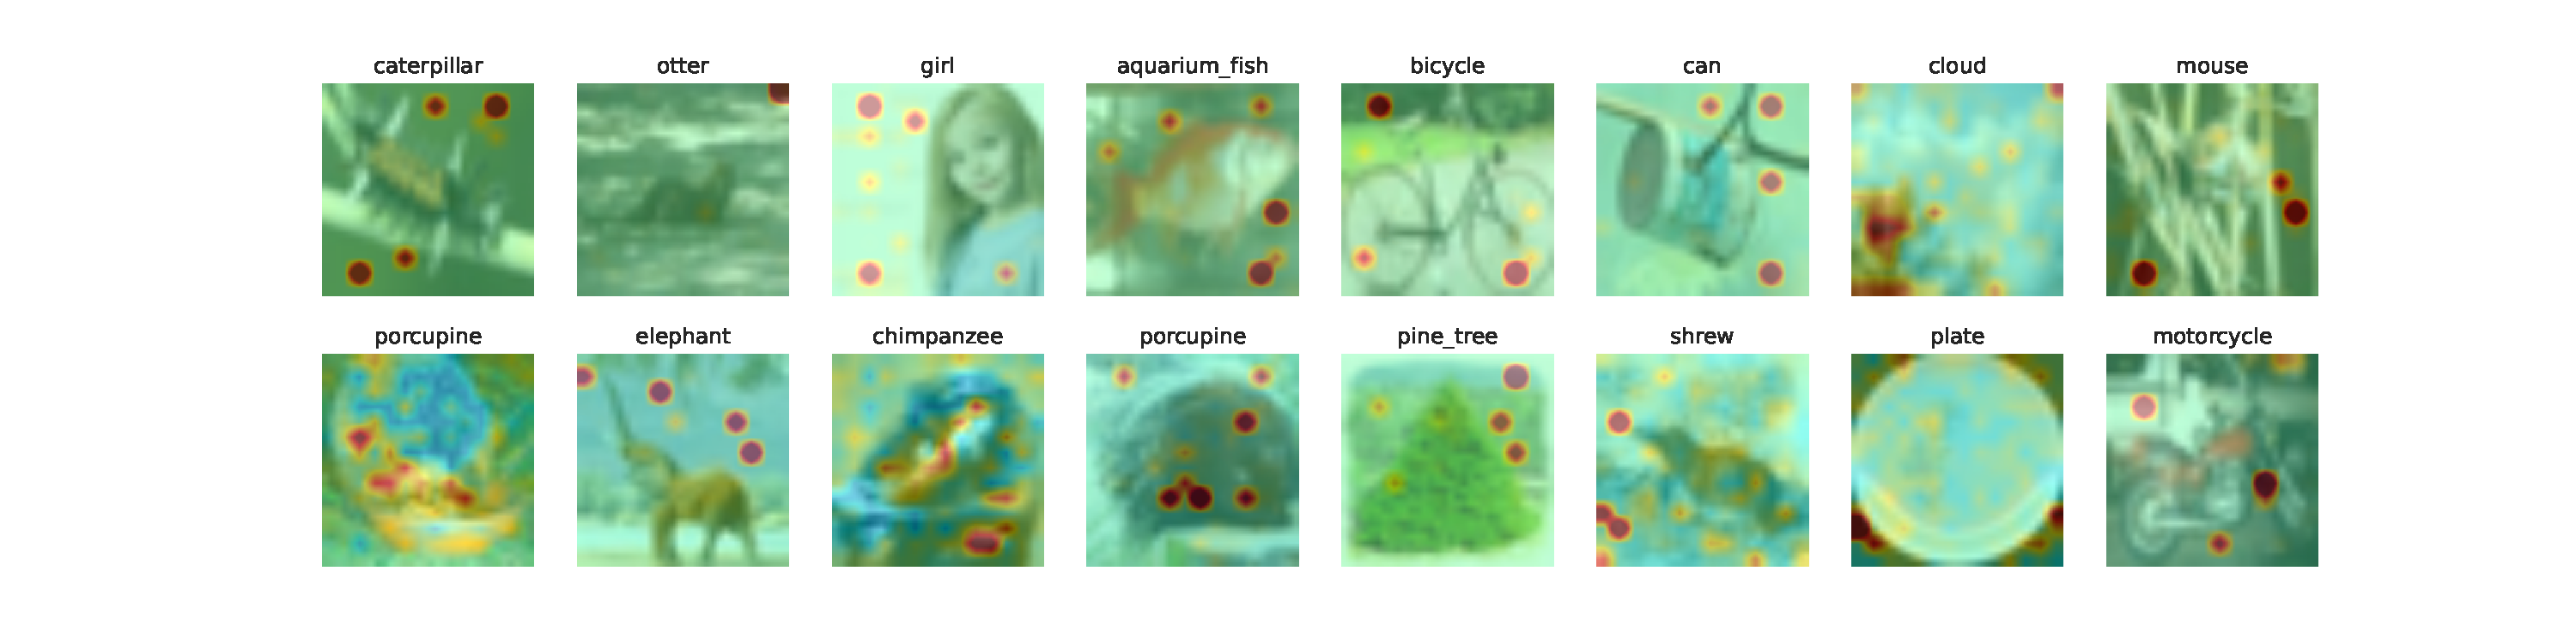
\includegraphics[width=\linewidth]{images/cifar100_vit_base_patch16_224_noproxy_0.pdf}
            \caption{Without Proxy Attention}
        \end{subfigure}
        \begin{subfigure}[b]{1\textwidth}
            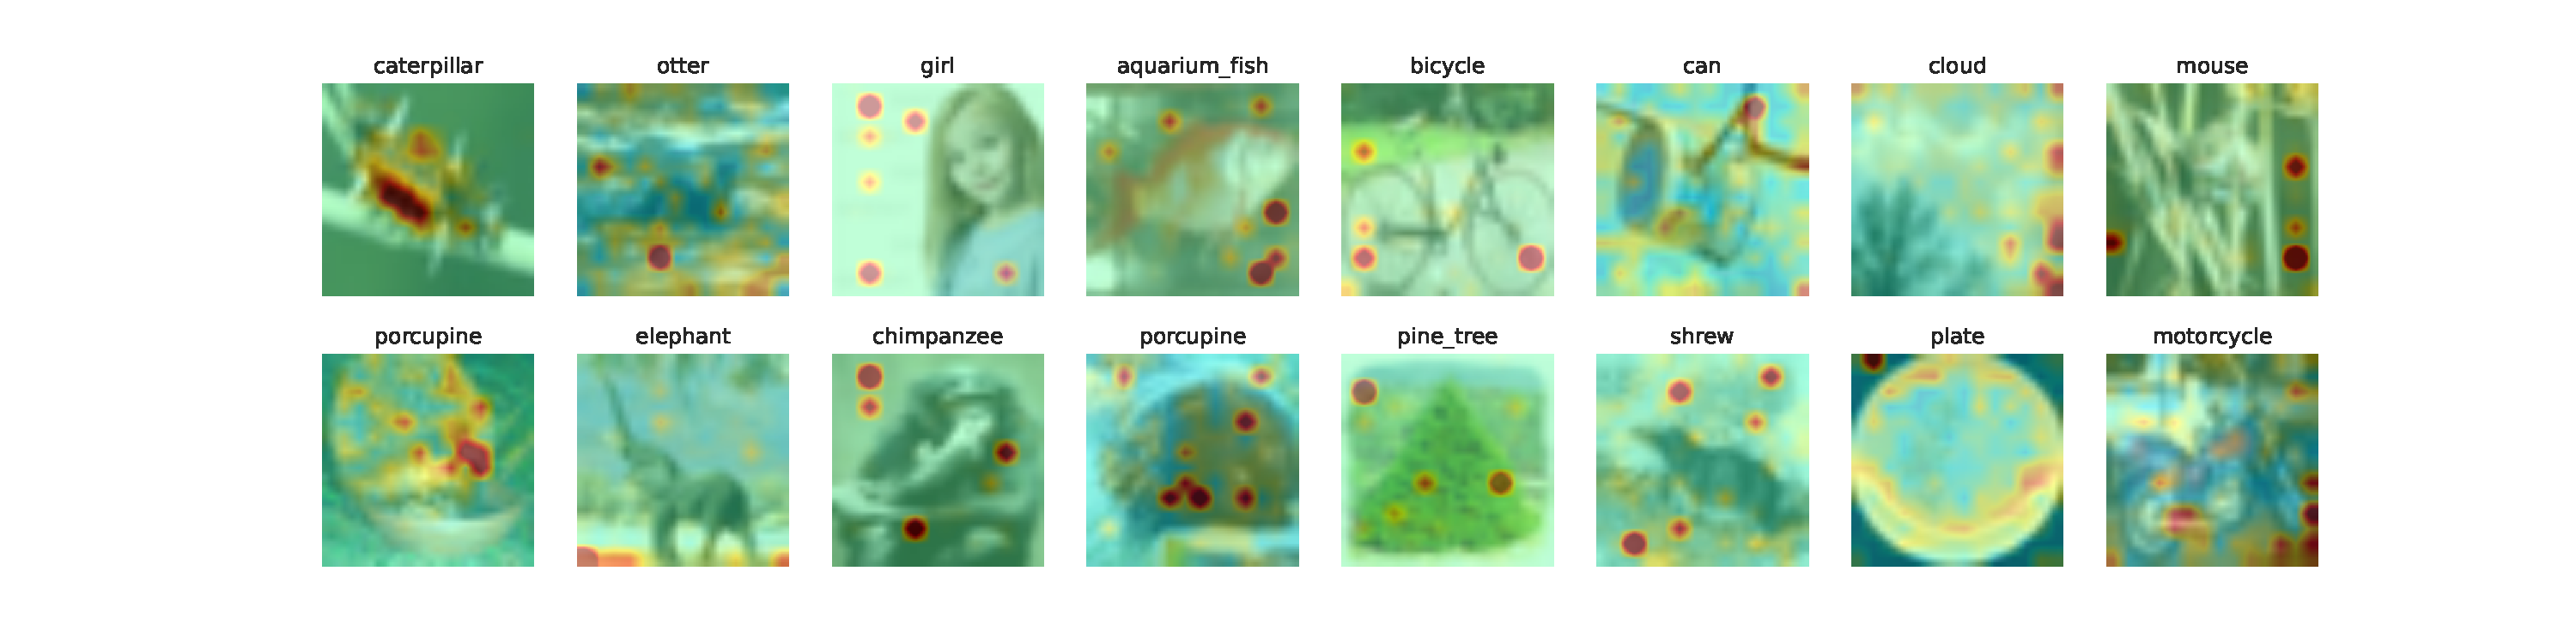
\includegraphics[width=\linewidth]{images/cifar100_vit_base_patch16_224_proxy_0.pdf}
            \caption{With Proxy Attention}
        \end{subfigure}
        \caption{Comparison of attention maps generated by vit\_base\_patch16\_224 trained with and without Proxy Attention on the cifar100 dataset}
        \label{fig:vit_cifar100}
    \end{figure}
    


\subsection{Tsinghua Dogs, ResNet50 , GradCamPlusPlus}
This section explores the explainability of the ResNet50 \cite{heDeepResidualLearning2016} trained with and without Proxy Attention on the Tsinghua dogs dataset \cite{zouNewDatasetDog2020}. The results are shown in Figure \ref{fig:resnet50_tsing}. The attention maps were generated using GradCamPlusPlus \cite{chattopadhayGradCAMGeneralizedGradientBased2018}.

Both the models in this case were accurate enough for the results to be similar. In the case of the second column of images, the model trained with proxy attention seemed to localize the position of the dogs better.  In a few of the other examples of the model trained with proxy attention, more focus is placed on the faces of the dogs, which would probably have helped the model recognize the breeds better.

\begin{figure}[!htb]
    \begin{subfigure}[b]{1\textwidth}
        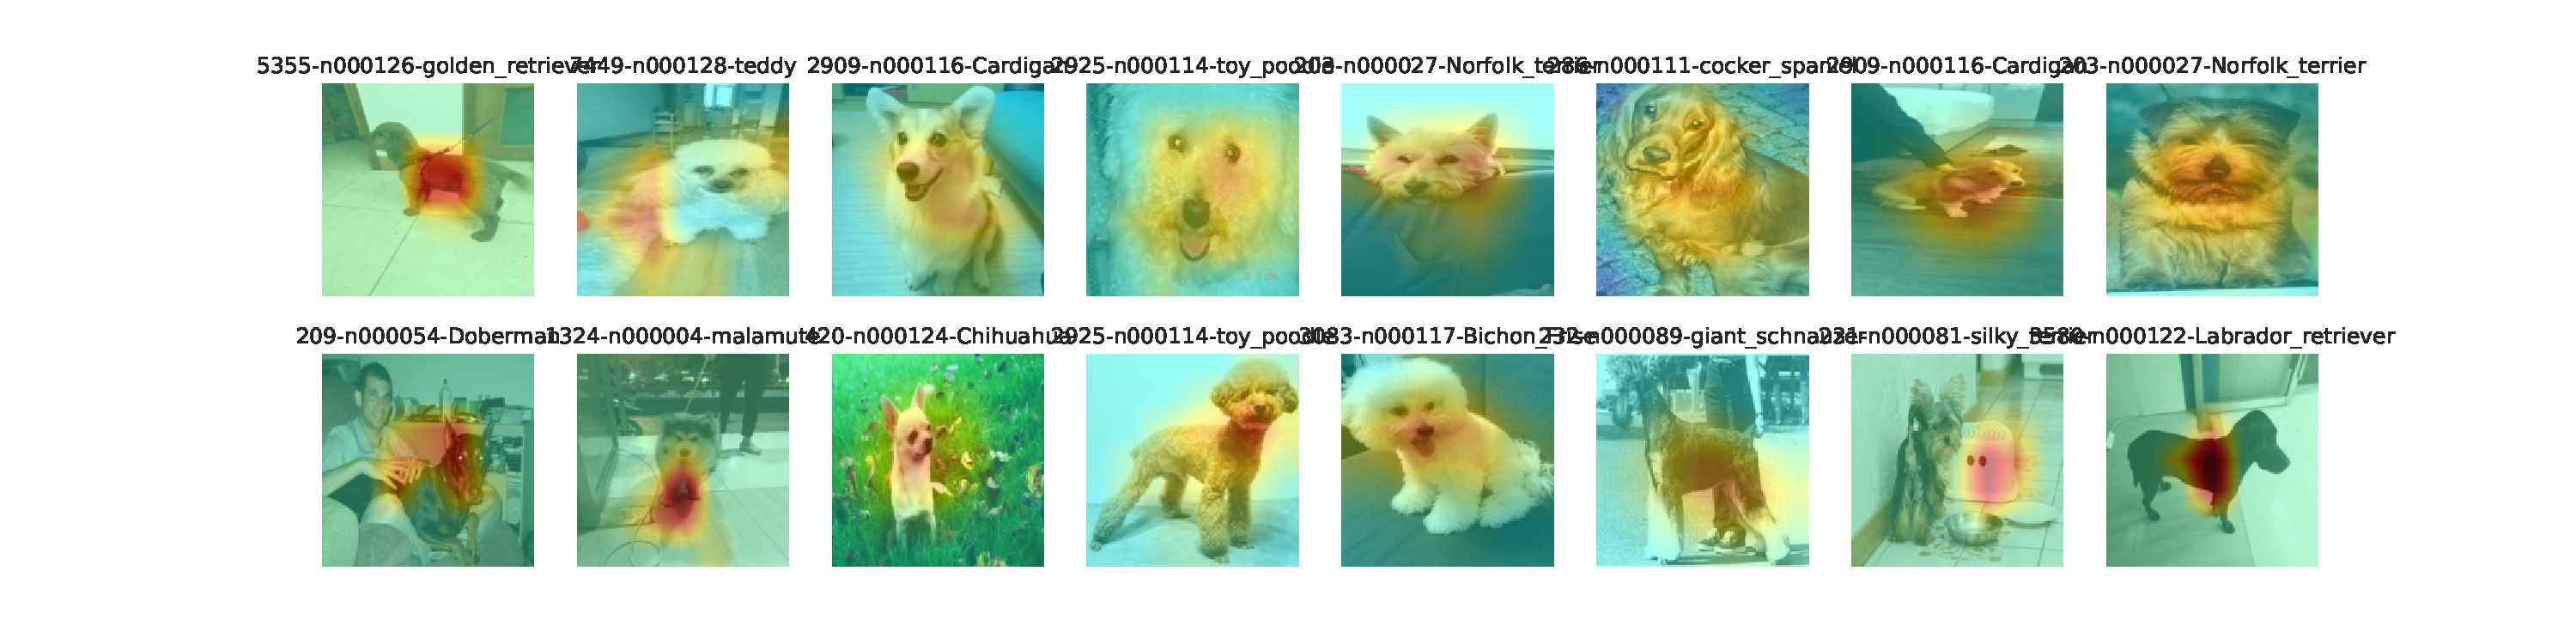
\includegraphics[width=\linewidth]{images/gpp_tsing_resnet50_noproxy_0.pdf}
        \caption{Without Proxy Attention}
    \end{subfigure}
    \begin{subfigure}[b]{1\textwidth}
        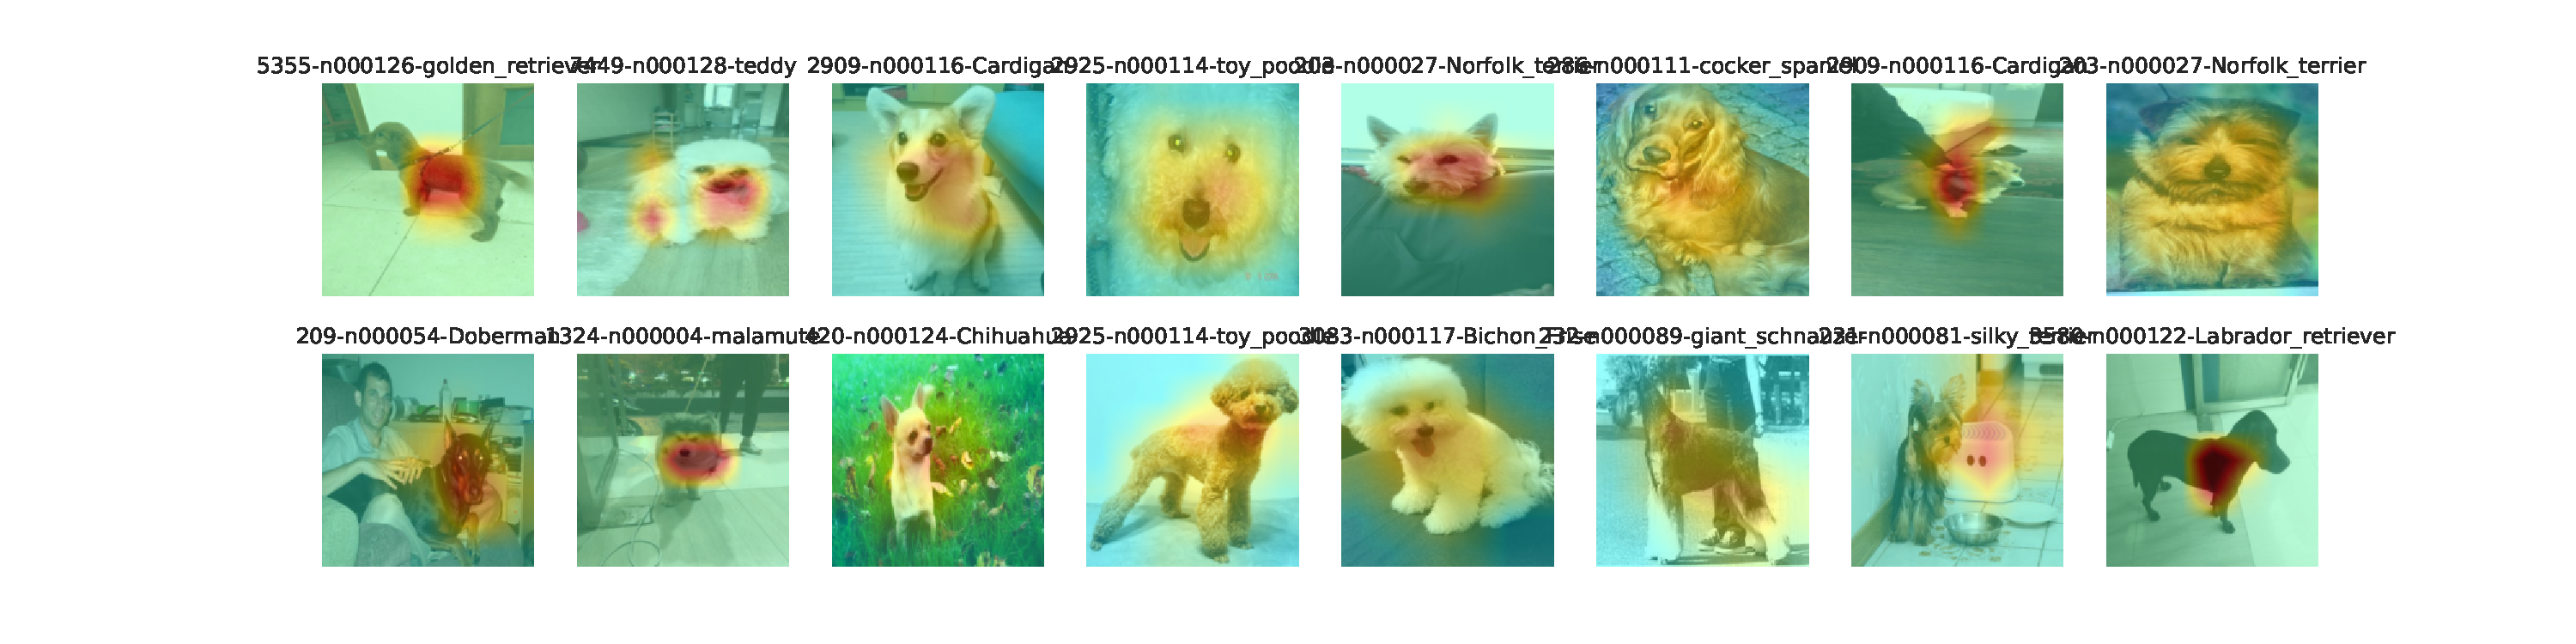
\includegraphics[width=\linewidth]{images/gpp_tsing_resnet50_proxy_0.pdf}
        \caption{With Proxy Attention}
    \end{subfigure}
    \caption{Comparison of attention maps generated by resnet50 trained with and without Proxy Attention on the tsing dataset}
    \label{fig:resnet50_tsing}
\end{figure}


\subsection{Tsinghua Dogs, ResNet18, EigenGradCAM}
This section explores the explainability of the ResNet18 \cite{heDeepResidualLearning2016} trained with and without Proxy Attention on the Tsinghua dogs dataset \cite{zouNewDatasetDog2020}. The results are shown in Figure \ref{fig:resnet18_tsing}. The attention maps were generated using EigenGradCAM \cite{banymuhammadEigenCAMVisualExplanations2021}.

The results obtained for this comparison are also similar to the ones above. In some cases, though, the model trained with proxy attention seemed to learn the wrong part of the image, even though it had initially got it correct.

\begin{figure}[!htb]
    \begin{subfigure}[b]{1\textwidth}
        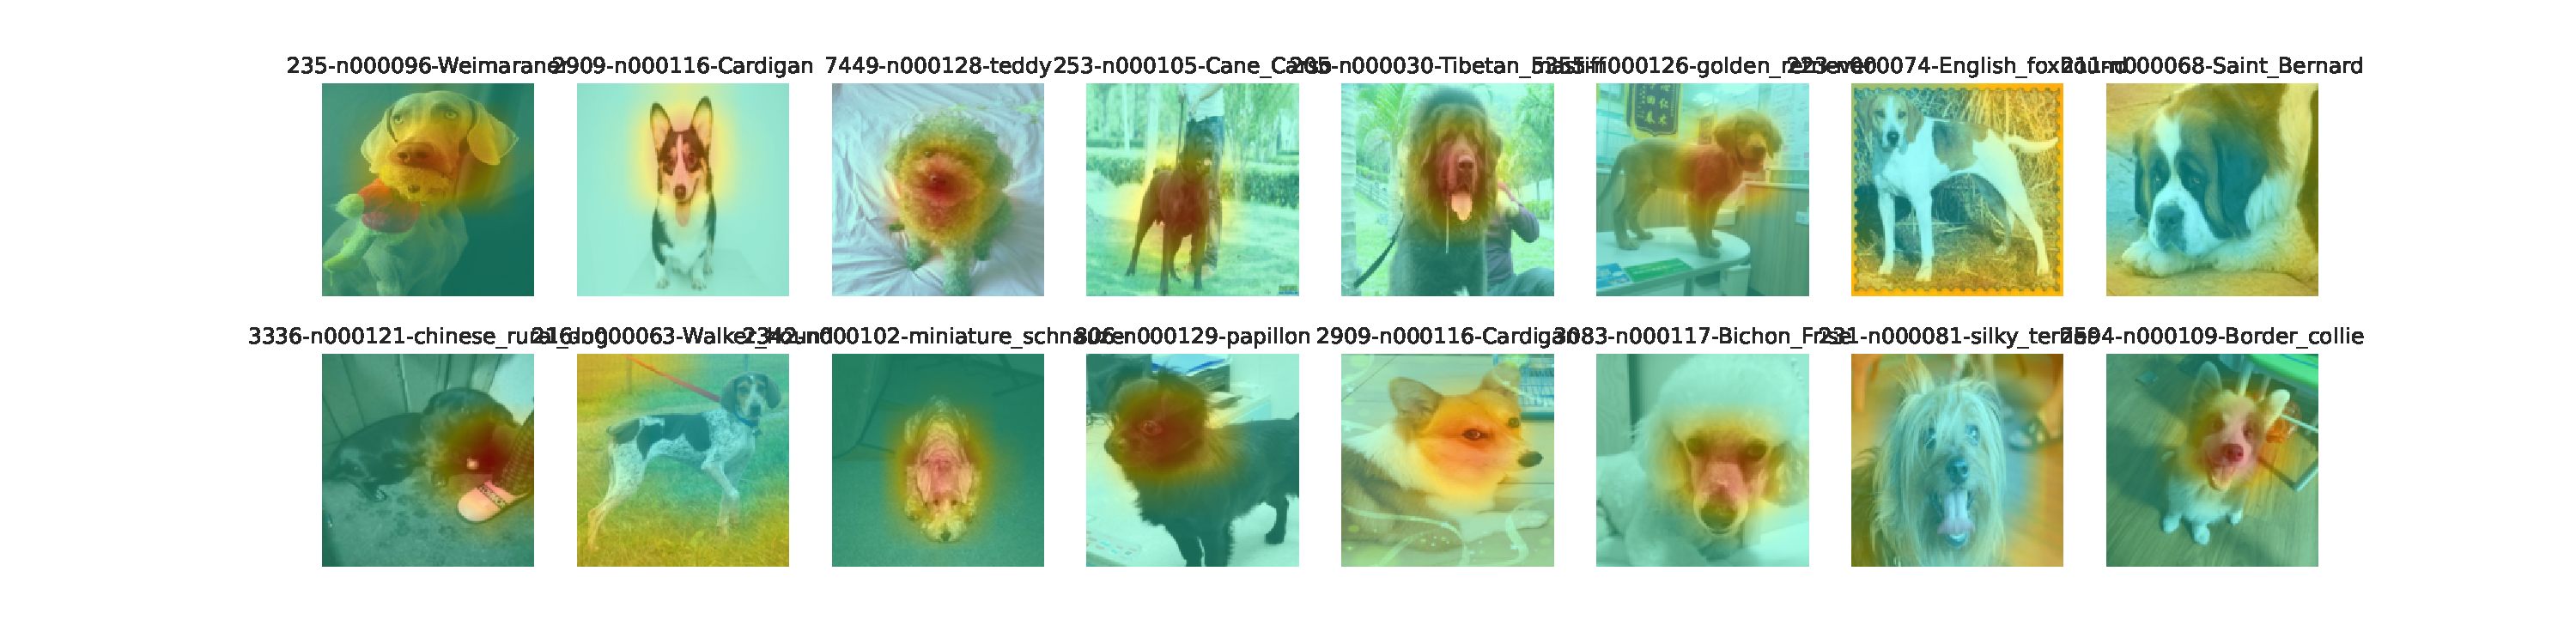
\includegraphics[width=\linewidth]{images/tsing_resnet18_noproxy_0.pdf}
        \caption{Without Proxy Attention}
    \end{subfigure}
    \begin{subfigure}[b]{1\textwidth}
        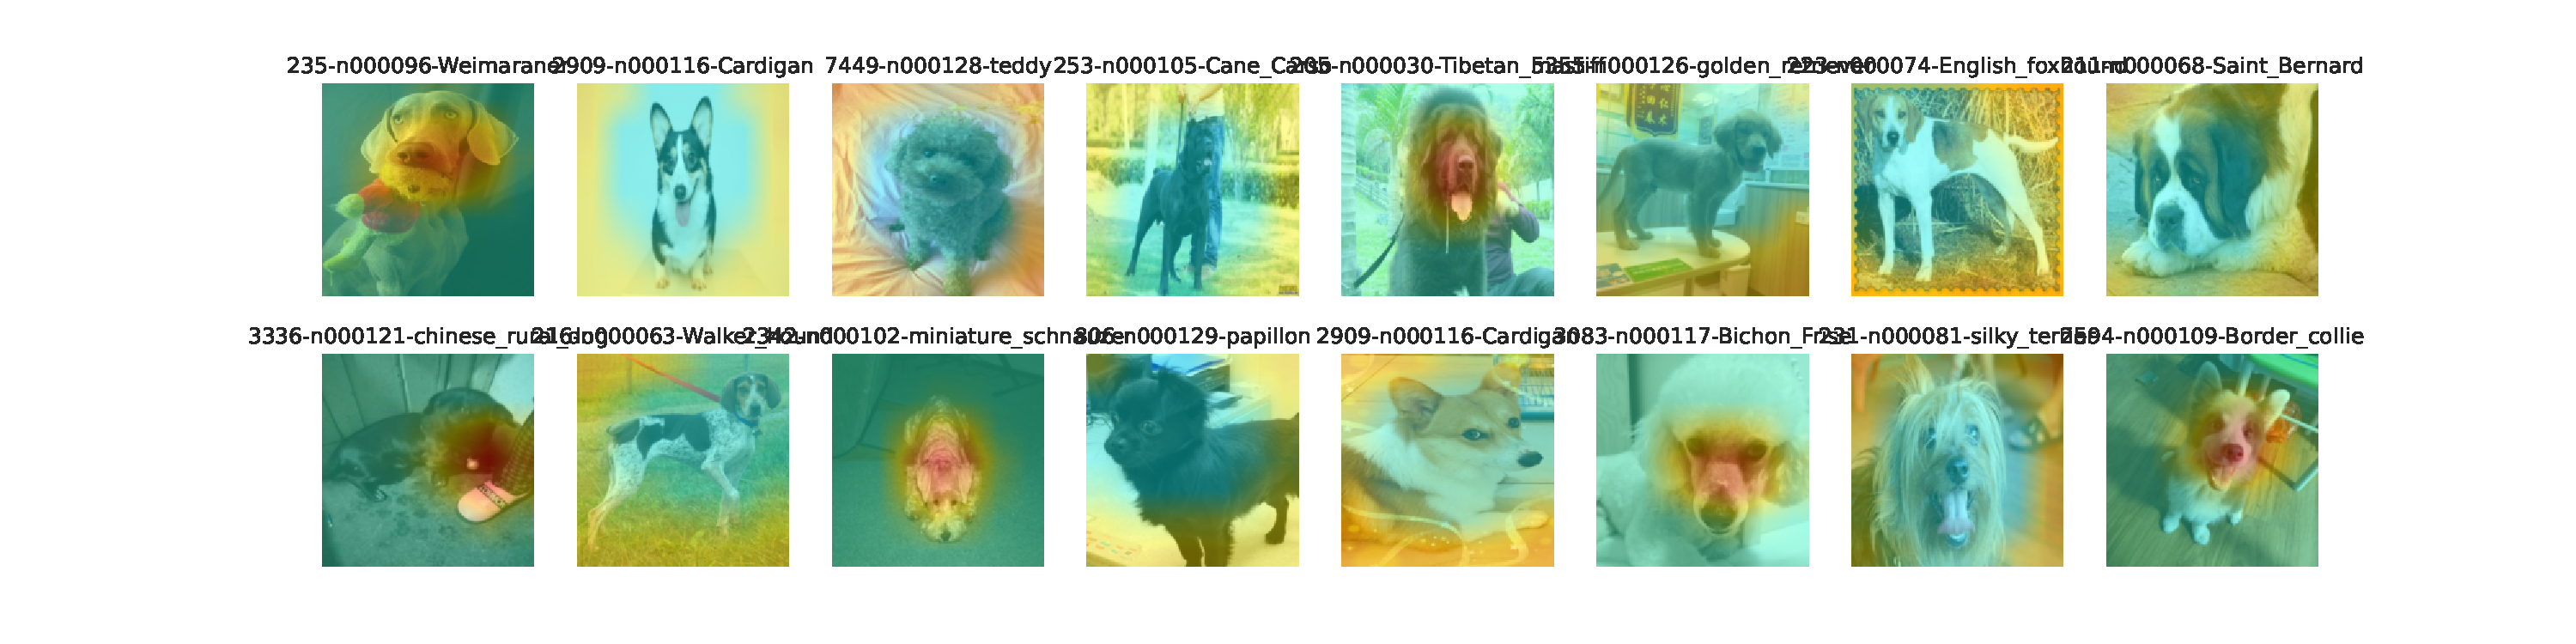
\includegraphics[width=\linewidth]{images/tsing_resnet18_proxy_0.pdf}
        \caption{With Proxy Attention}
    \end{subfigure}
    \caption{Comparison of attention maps generated by resnet18 trained with and without Proxy Attention on the tsing dataset}
    \label{fig:resnet18_tsing}
\end{figure}



